\documentclass{statsoc}
\usepackage[utf8]{inputenc}
\usepackage[english]{babel}
\usepackage[a4paper]{geometry}
%\usepackage{paralist}
%\usepackage{enumitem}
\usepackage{bm}
\usepackage{amsmath}
\usepackage{amssymb}
%%\usepackage{graphics}
\usepackage[authoryear]{natbib}
\usepackage{relsize}
%\usepackage{color}
\usepackage[table]{xcolor}
\usepackage{multirow}
\usepackage{mathptmx}
%\usepackage{transparent}
%\usepackage{xcolor}
%\usepackage{efbox}
\usepackage{float}
%\usepackage{subfig}
%
%\usepackage{hvfloat}
%\usepackage{booktabs}
%\usepackage[font=footnotesize]{caption}
\usepackage{etoolbox}
\usepackage{url}
\usepackage[table]{xcolor}
\usepackage{array}
\usepackage{tikz}
\usetikzlibrary{trees}
\DeclareGraphicsExtensions{.pdf,.png,.jpg,.eps} 
\usepackage[ruled]{algorithm2e}
 \definecolor{algobackgroup}{gray}{0.05}

\makeatletter
\patchcmd{\@makecaption}
{\parbox}
{\advance\@tempdima-\fontdimen2\font\parbox} % decrease the width!
{}{}
\makeatother  

\usepackage{graphicx}
\usepackage[caption=false]{subfig}
\usepackage{enumerate}
\usepackage{comment}
\usepackage{float}

\newcommand\Pair[4]{%
  \arrayrulecolor{cyan!60!black!40}%
  \arrayrulewidth=1pt
  \renewcommand\extrarowheight{1.5pt}%
  \begin{tabular}{|p{2cm}|>{\centering\arraybackslash}p{10pt}|}
  \hline
  \rowcolor{cyan!60!black!10}\textcolor{red!60!black}{#1} & \textcolor{red!60!black}{#2} \\
  \hline 
  \rowcolor{cyan!60!black!10}\textcolor{red!60!black}{#3} & \textcolor{red!60!black}{#4} \\
  \hline
  \end{tabular}%
}


\pagenumbering{Roman}
\renewcommand\thefigure{\Roman{figure}}


\newtheorem{thm}{Theorem}

\title[]{Electronic Supplementary Material for the paper: `A Bayesian Quest for Finding a Unified Model for Predicting Volleyball Games'}
\author[Egidi and Ntzoufras]{Leonardo Egidi}
\address{Dipartimento di Scienze Economiche, Aziendali, Matematiche e Statistiche `Bruno de Finetti',
	Universit\`{a} degli Studi di Trieste,
	Trieste,
	Italy.}
\email{legidi@units.it}
\author[Egidi and Ntzoufras]{Ioannis Ntzoufras}
\address{AUEB Sports Analytics Group, Computational and Bayesian Statistics Lab, Department of Statistics,
	Athens University of Economics and Business,
	Athens, Greece.}
\email{ntzoufras@aueb.gr}
 
 


\begin{document}

\maketitle



\section*{Sensitivity analysis}

To account for robustness in our posterior estimates, we performed some sensitivity tests for the model's parameters (see Table 4 in the paper for a comprehensive summary of the final selected model). Sensitivity plots may be retrieved in the Supplementary Material folder available at \url{https://github.com/LeoEgidi/Bayesian-Volleyball-paper}. Specifically, we let vary: 


\begin{itemize}
\item the standard deviations of the normal priors for the parameters $\mu, \theta, H^{point}, H^{set}, m$
(first five panels in Figure~\ref{figS1});
\item  the scale parameter of the log-normal prior for $\lambda$ (sixth panel in Figure~\ref{figS1});
\item the inverse-gamma parameters $a_1, a_2, b_1, b_2$ for the hyper-priors $\tau^2_{\alpha} \sim \mathsf{InvGamma}(a_1,a_2), \ \tau^2_{\beta} \sim \mathsf{InvGamma}(b_1,b_2),$ assuming that the set and point abilities are assigned two normal priors, $\bm{\alpha} \sim \mathcal{N}(0, \tau^2_{\alpha}),\ \bm{\beta} \sim \mathcal{N}(0, \tau^2_{\beta}) $, respectively. For simplicity, we assume $a_1=a_2,\ b_1=b_2$ (Figures~\ref{figS3}--\ref{figS4}).
\end{itemize}
%
Red triangles on the $x$-axis in Figures~\ref{figS1} denote the values used in the final model. As a general comment, the posterior estimates seem to be not much sensitive with respect to the hyperparameters choices. All selected values seem to lie on the ``non-informative'' region where the priors are stabilized to a specific posterior solely based on data information. 

Regarding the point and set abilities in Figures~\ref{figS3}--\ref{figS4}, we note that there are not sensitive changes of the posterior estimates in correspondence of distinct hyperparameters' values of the inverse-gamma distributions for $\tau^2_{\alpha}, \tau^2_{\beta}$.

Then, according to these checks, we feel our analysis are robust enough to justify the hyperparameters' choices adopted in the paper.
%(see parameters $H^{point}, H^{set},m, \lambda$ and the overall averaged parameters $\overline{\alpha}, \overline{\beta}$). Regarding the parameters $\theta, \delta$ and $\gamma$, we note that the posterior uncertainty decreases as the standard deviations become smaller.

\begin{figure}
\centering
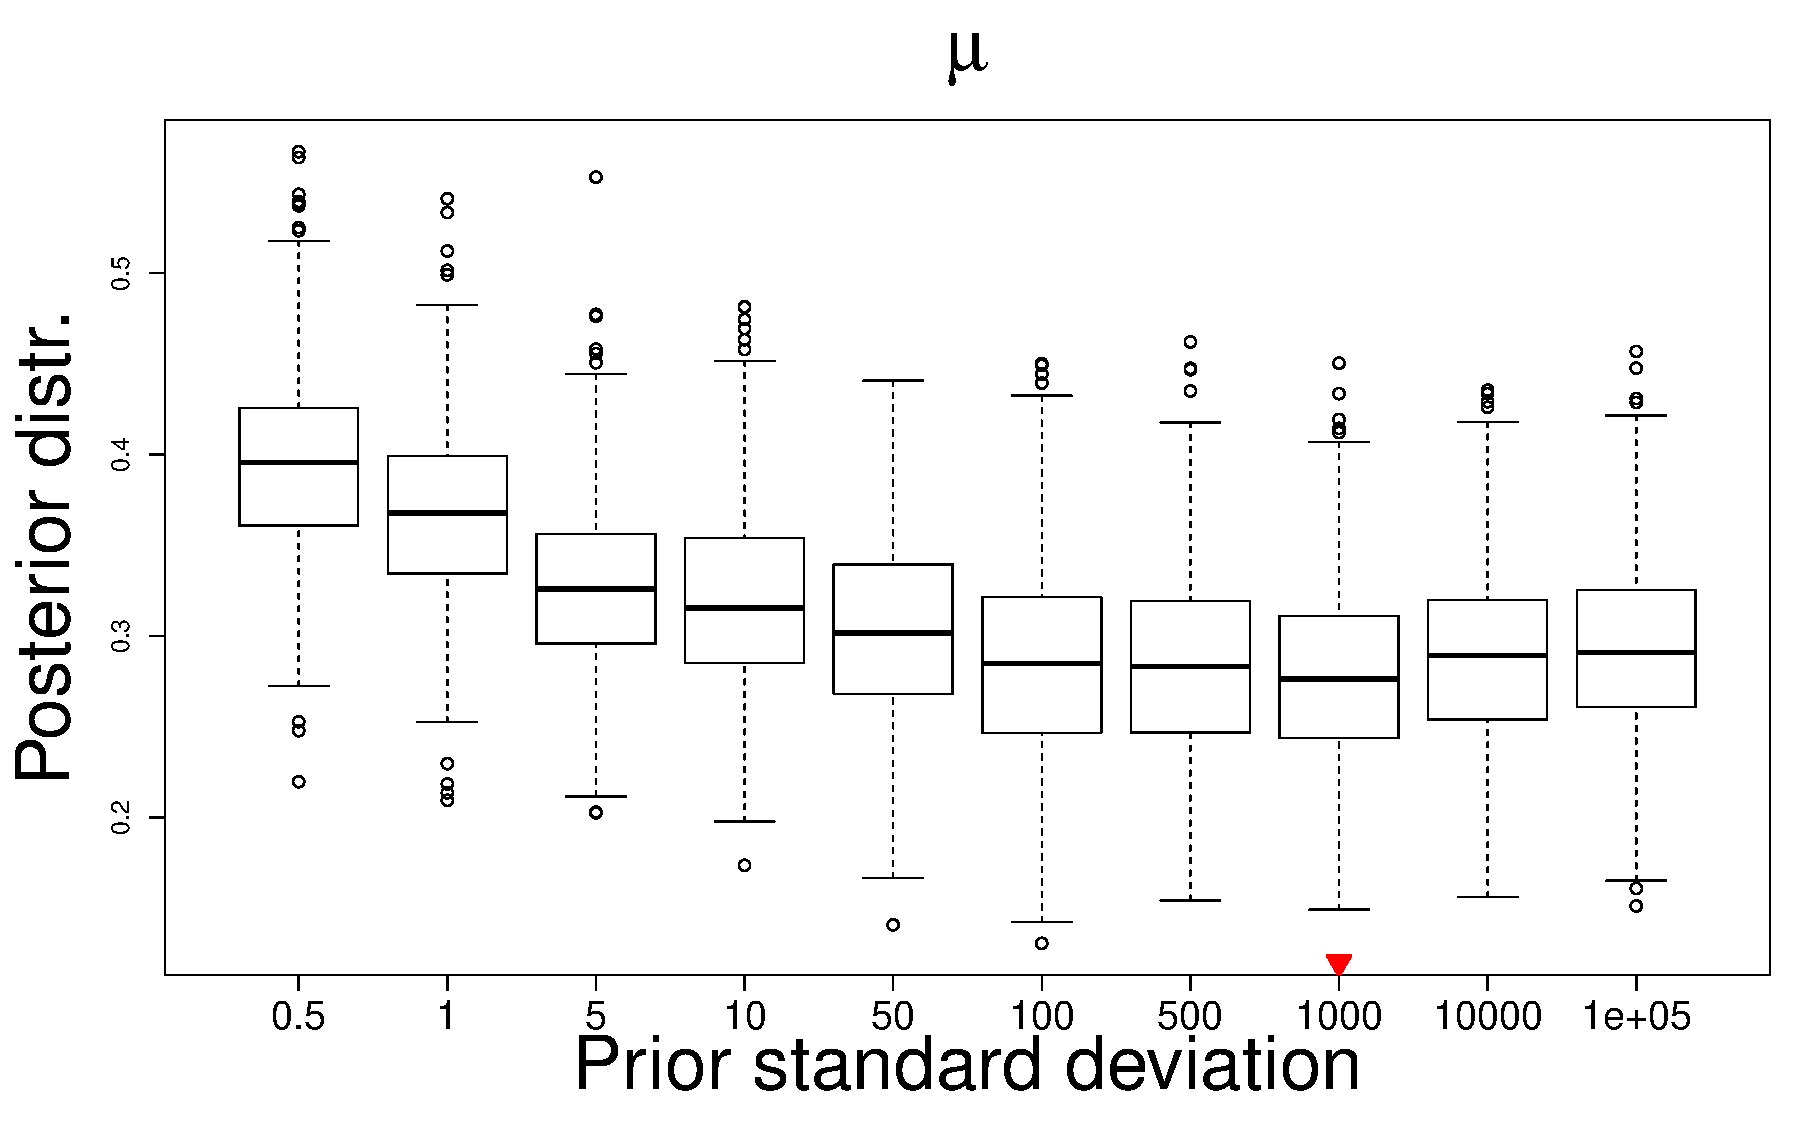
\includegraphics[scale=0.25]{Sensitivity/mu_sensitivity.pdf}~
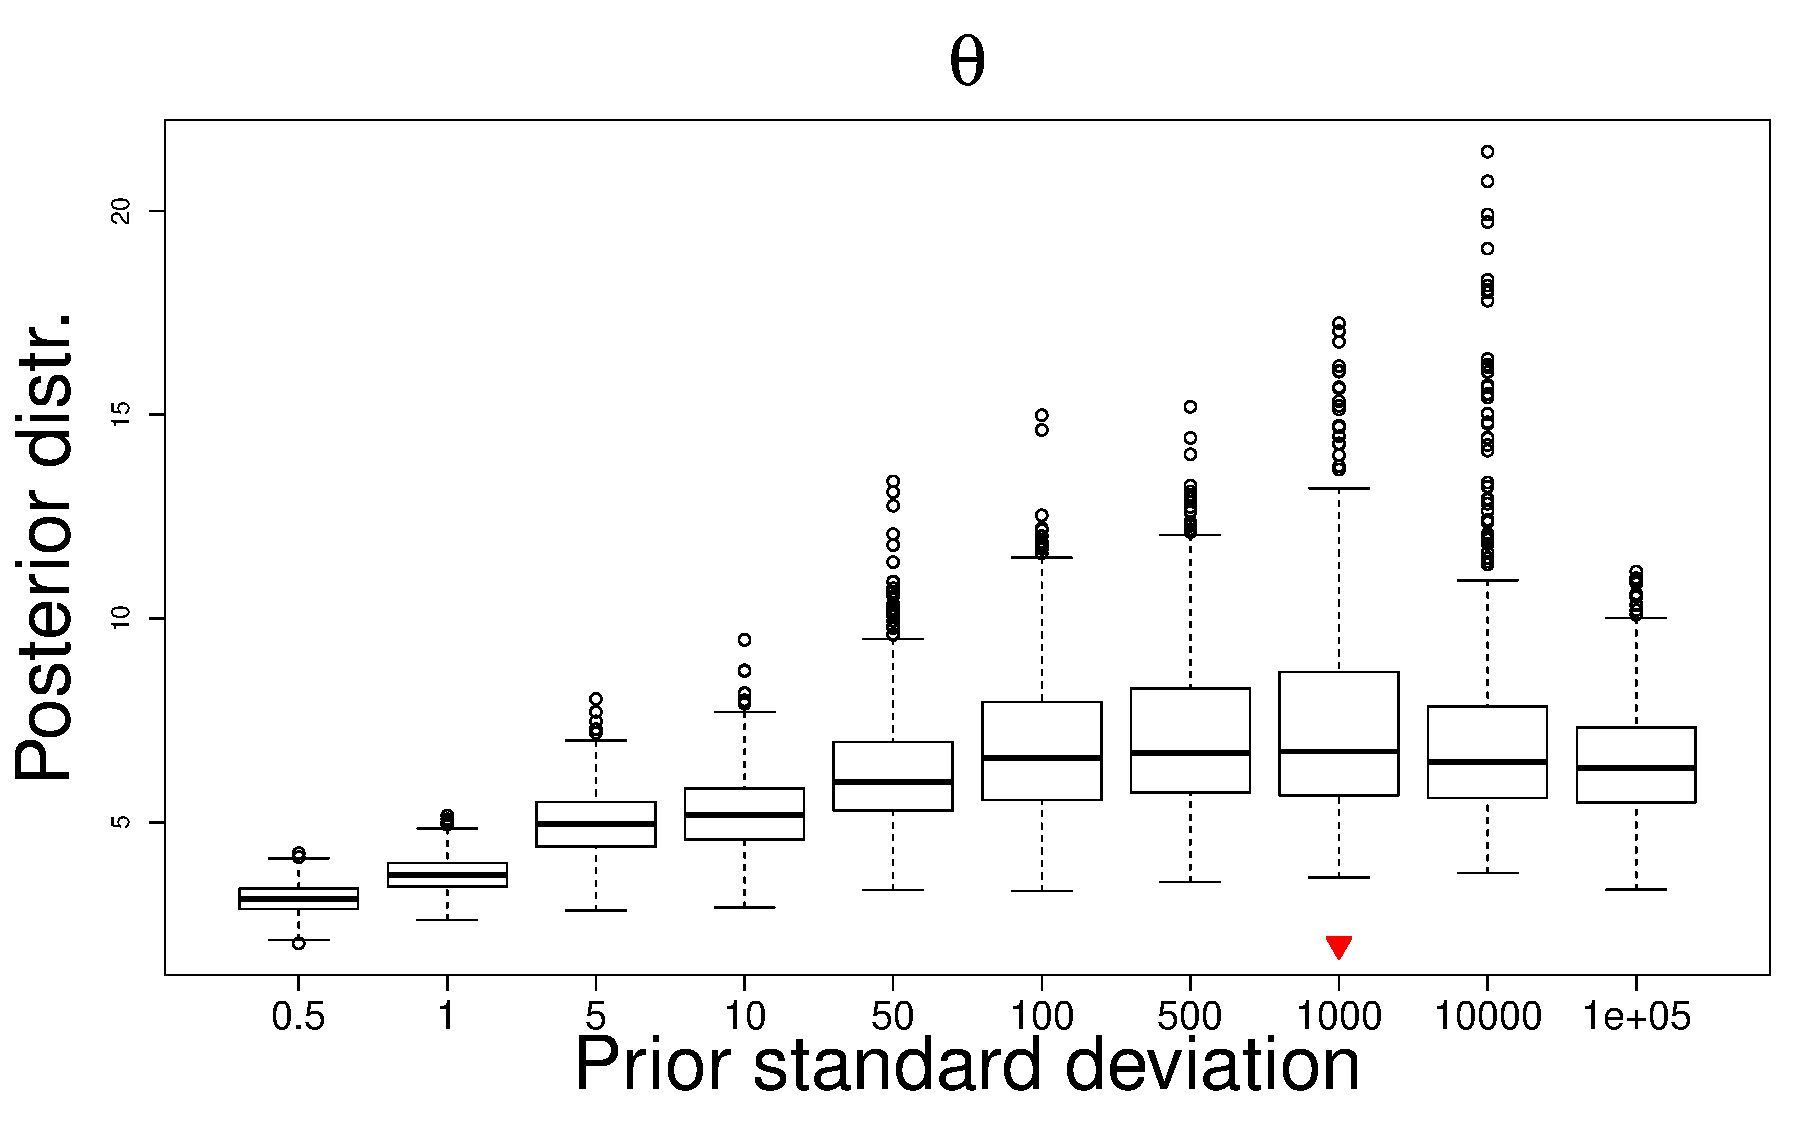
\includegraphics[scale=0.25]{Sensitivity/theta_sensitivity.pdf}\\
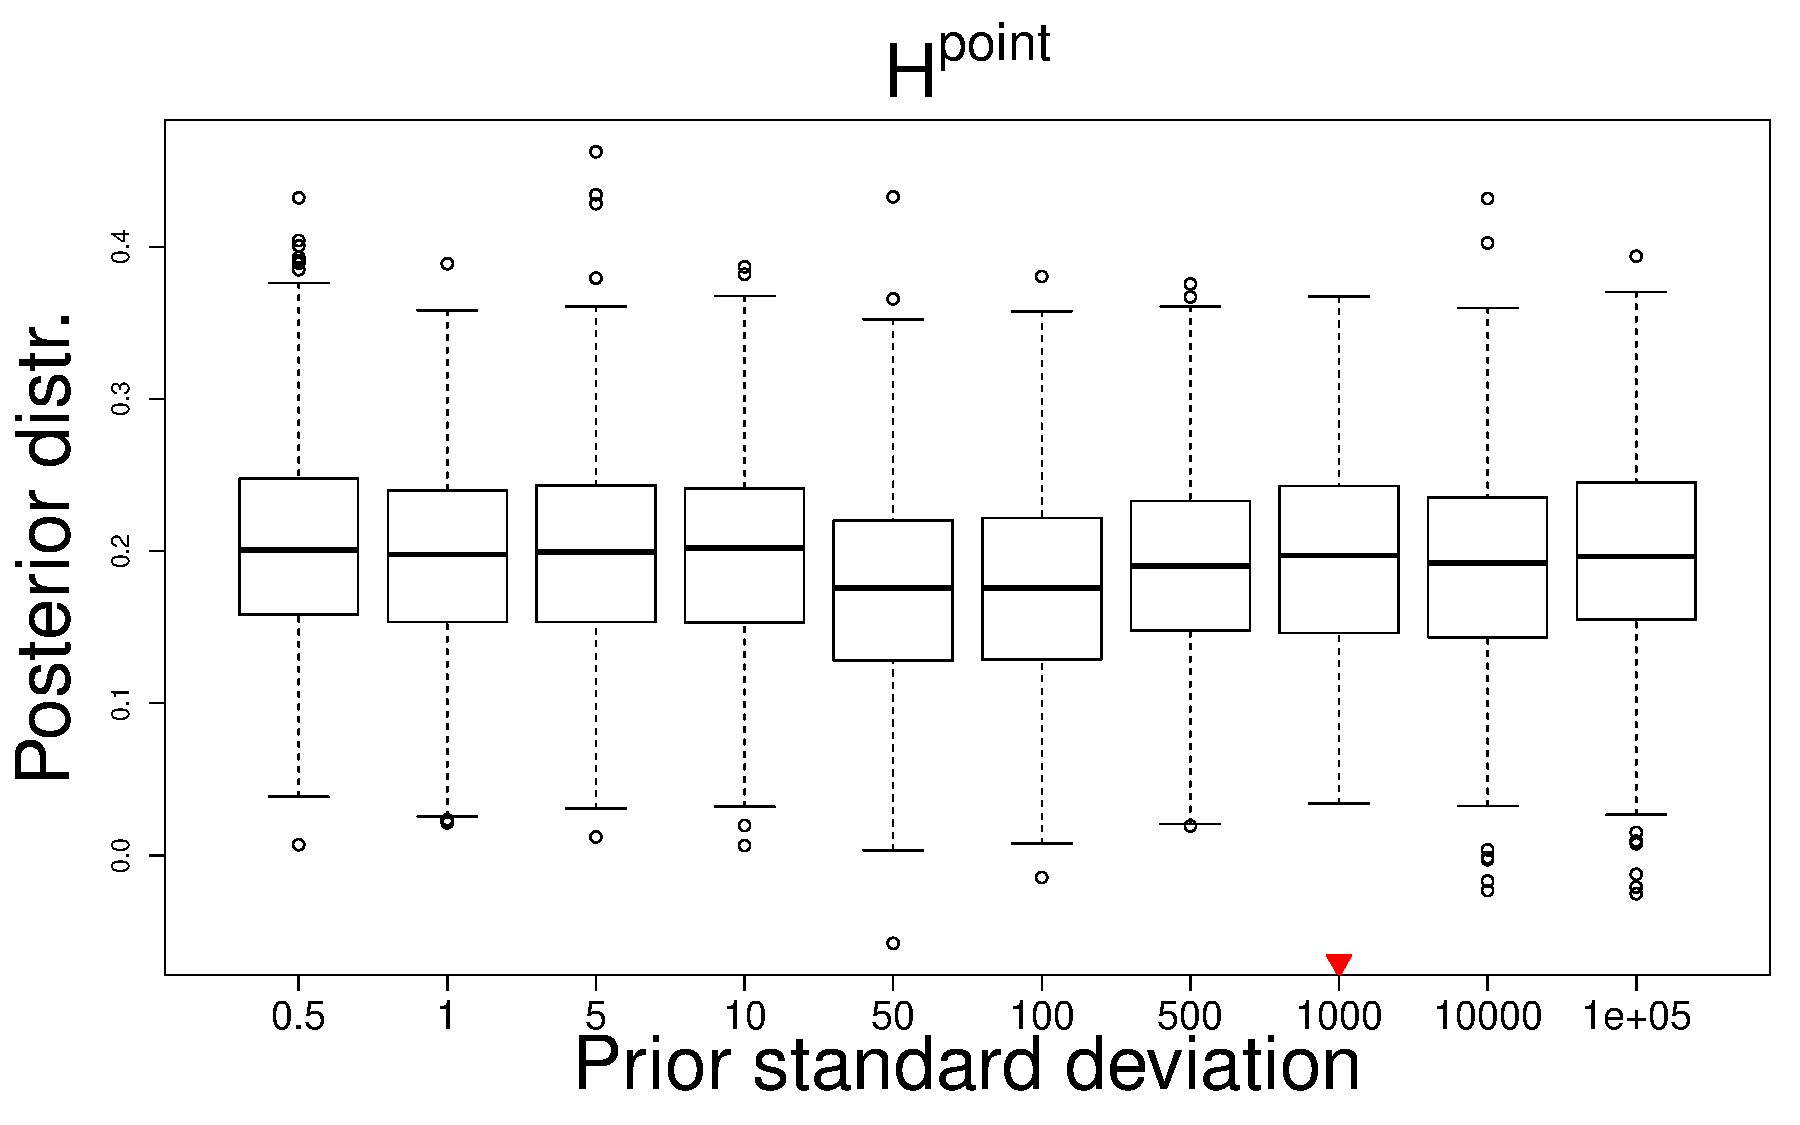
\includegraphics[scale=0.25]{Sensitivity/H_point_sensitivity.pdf}~
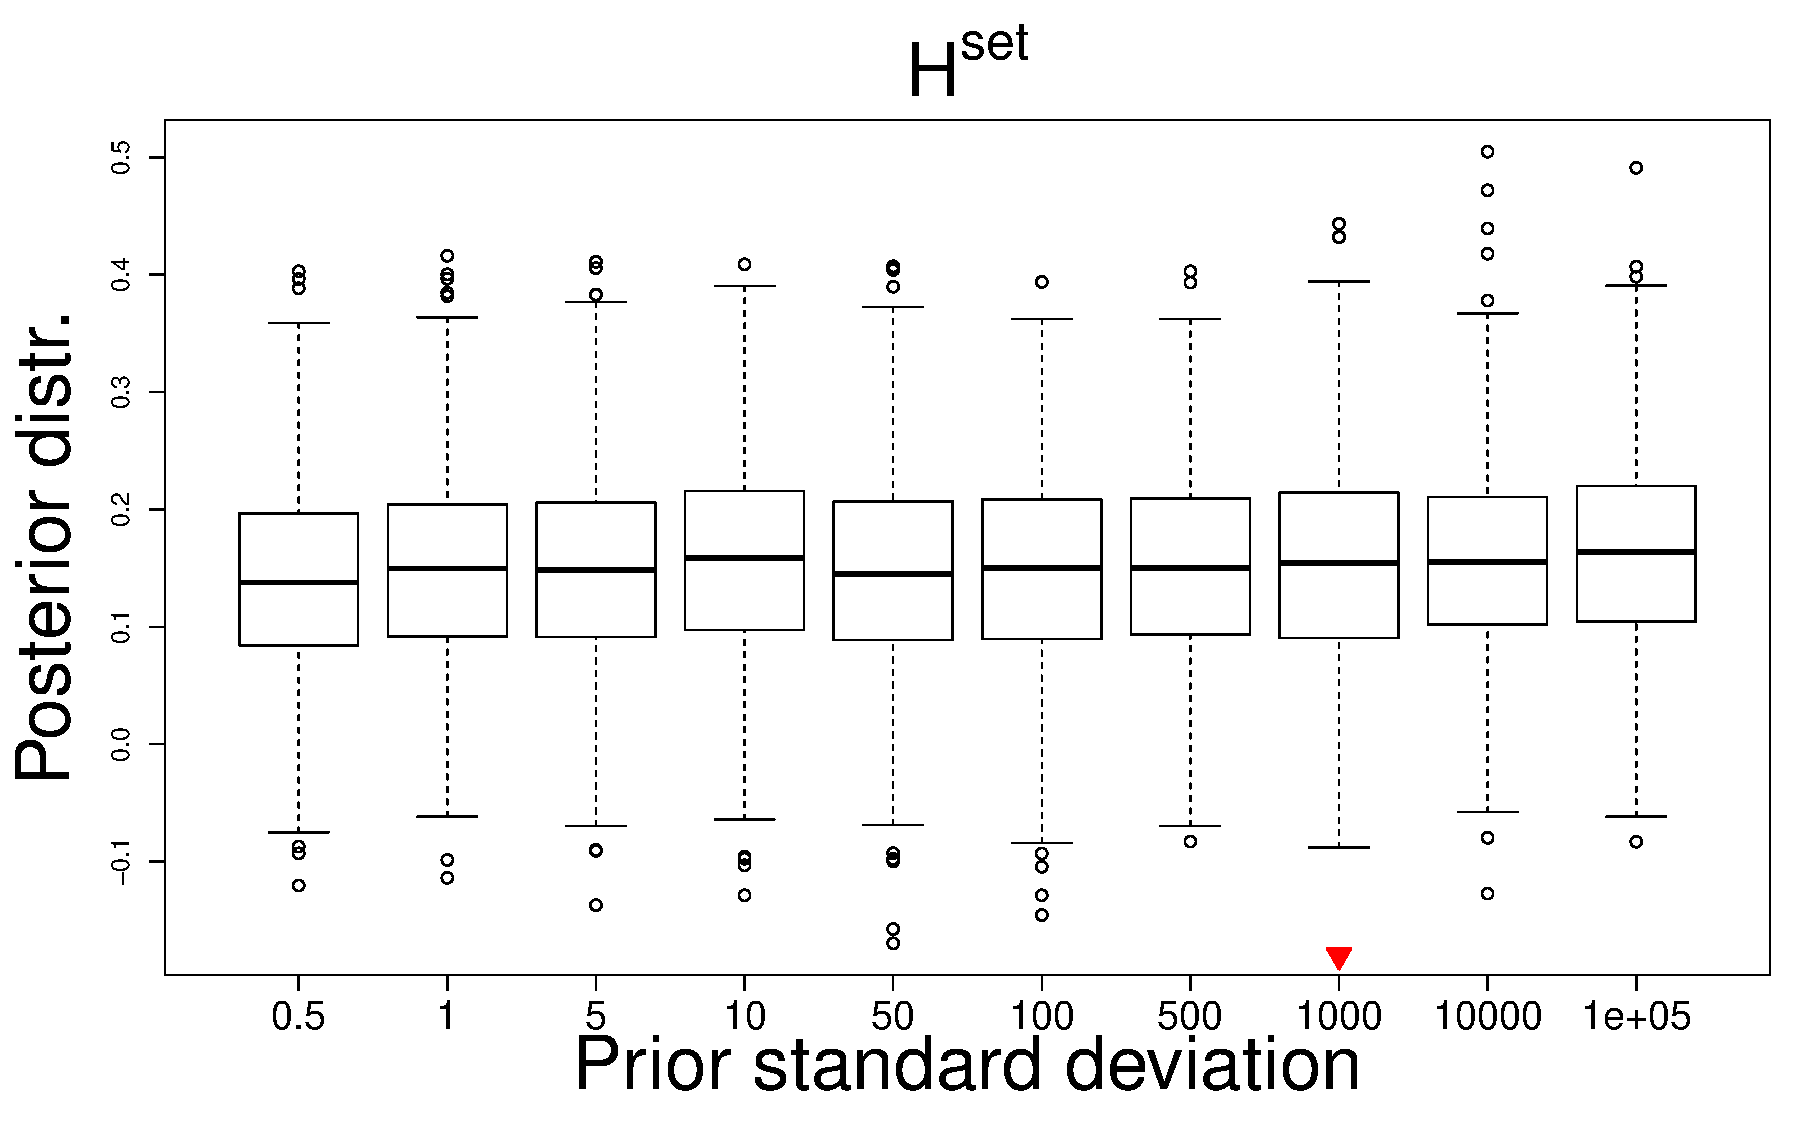
\includegraphics[scale=0.25]{Sensitivity/H_set_sensitivity.pdf}\\
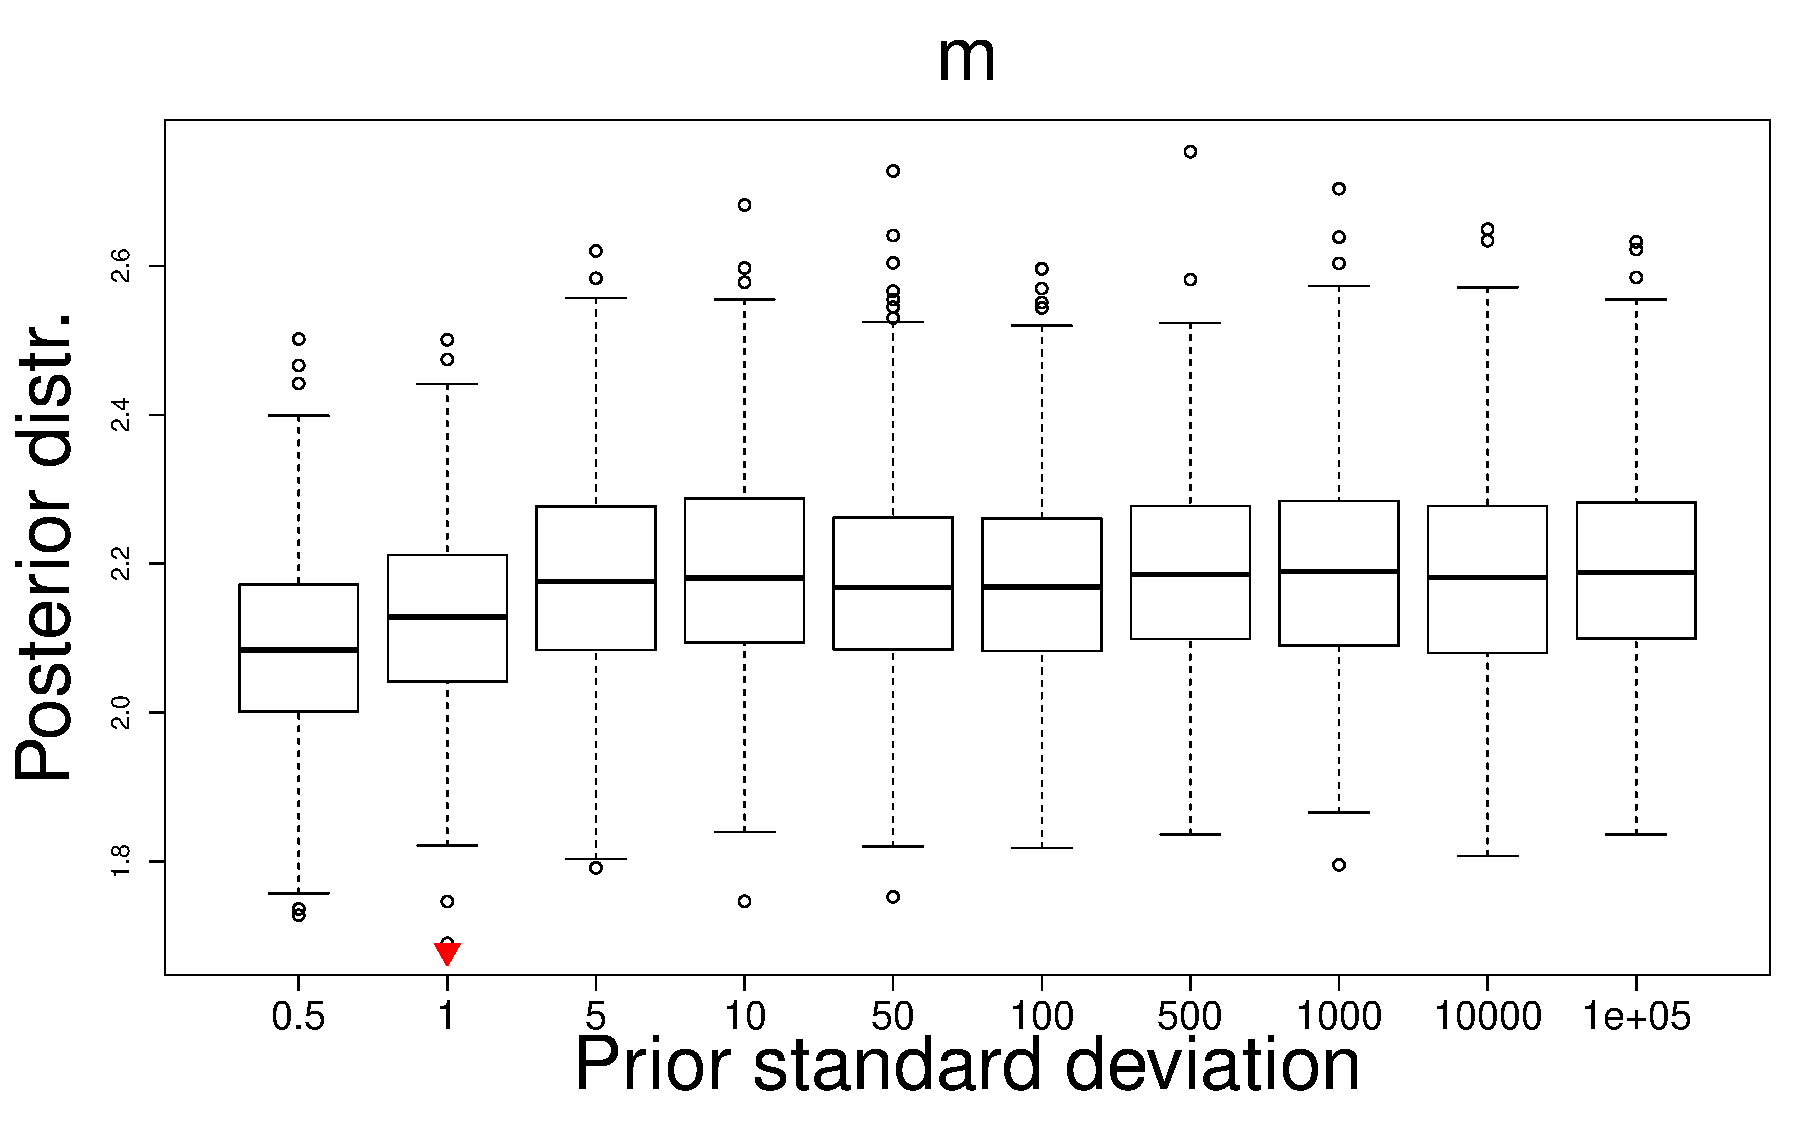
\includegraphics[scale=0.25]{Sensitivity/m_sensitivity.pdf}~
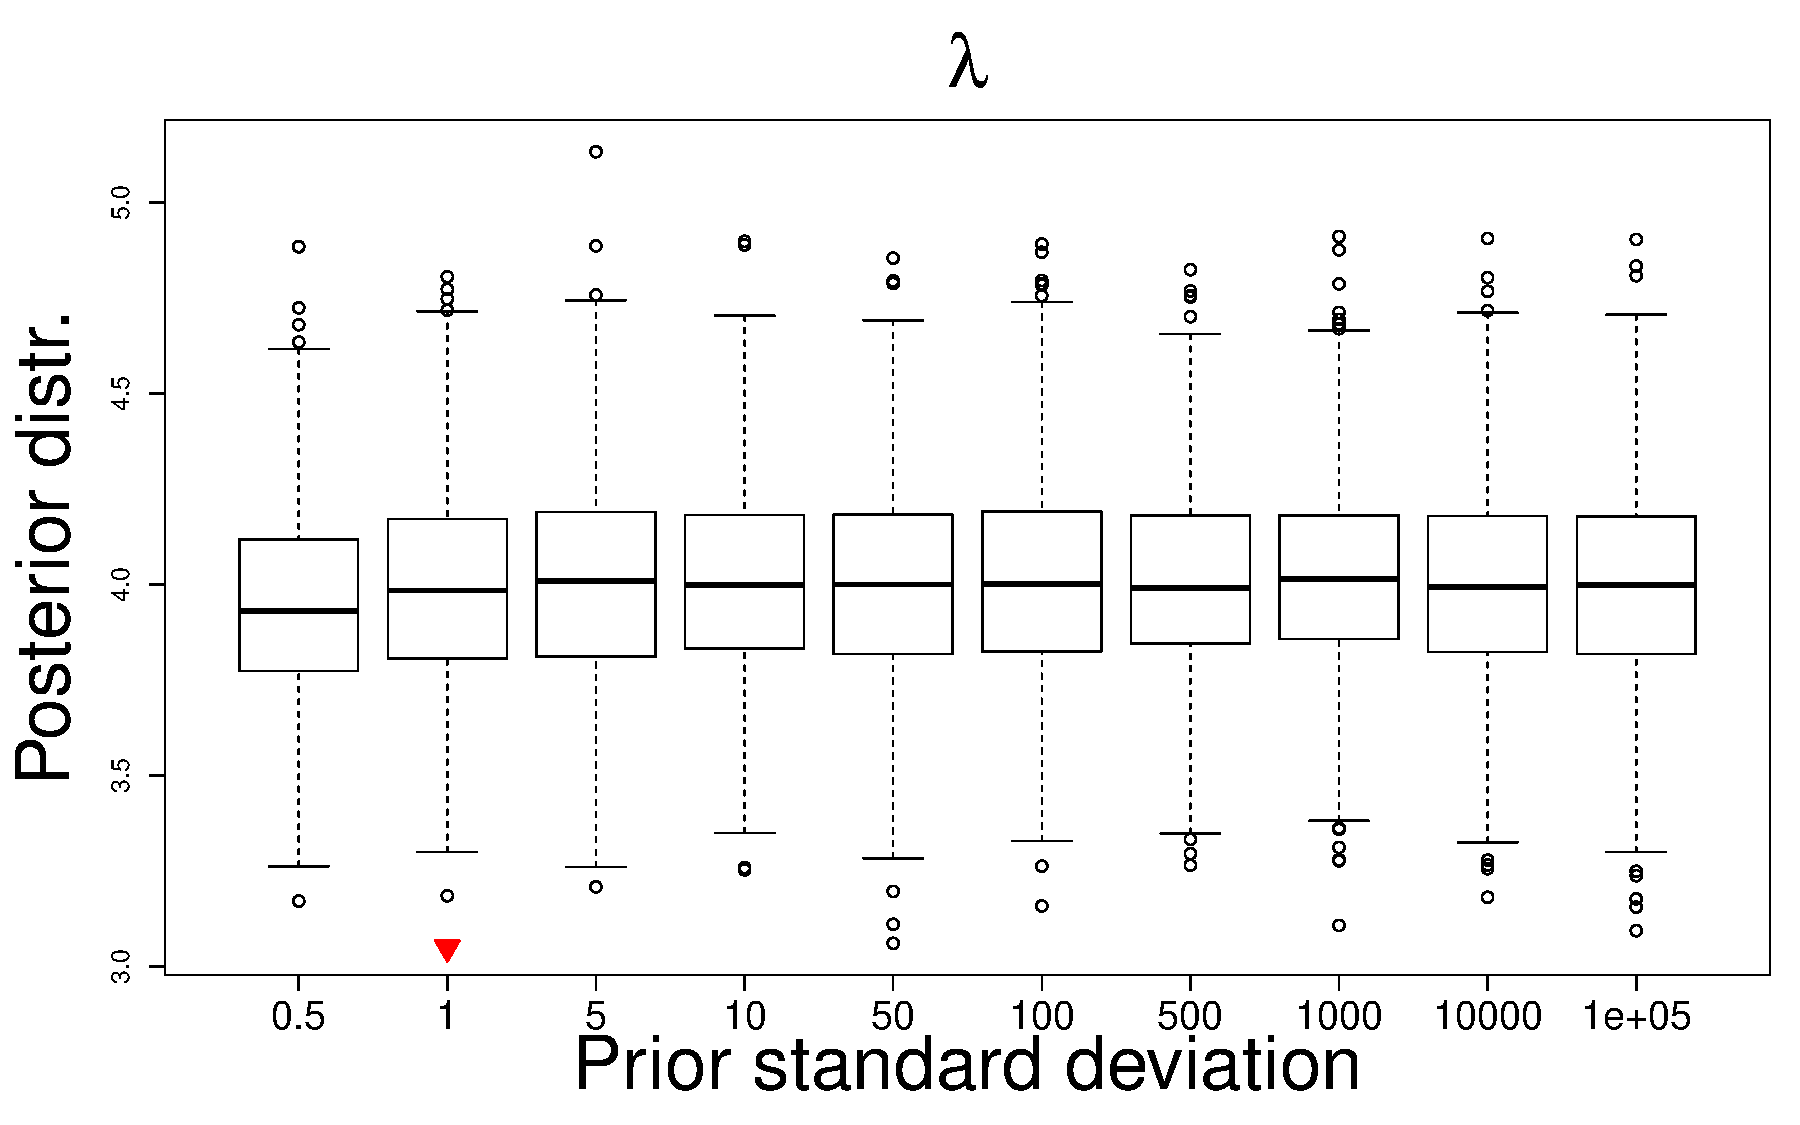
\includegraphics[scale=0.25]{Sensitivity/lambda_sensitivity.pdf}\\
\caption{Sensitivity tests for for the marginal posterior distributions of the parameters: $\mu, \theta, H^{point}, H^{set}, m, \lambda$ by varying the standard deviations of the normal priors and the scale parameter of the log-normal prior. {\tt rjags}, 1000 MCMC iterations, burn-in period of 100 iterations.}
\label{figS1}
\end{figure}
%


\begin{figure}
\centering
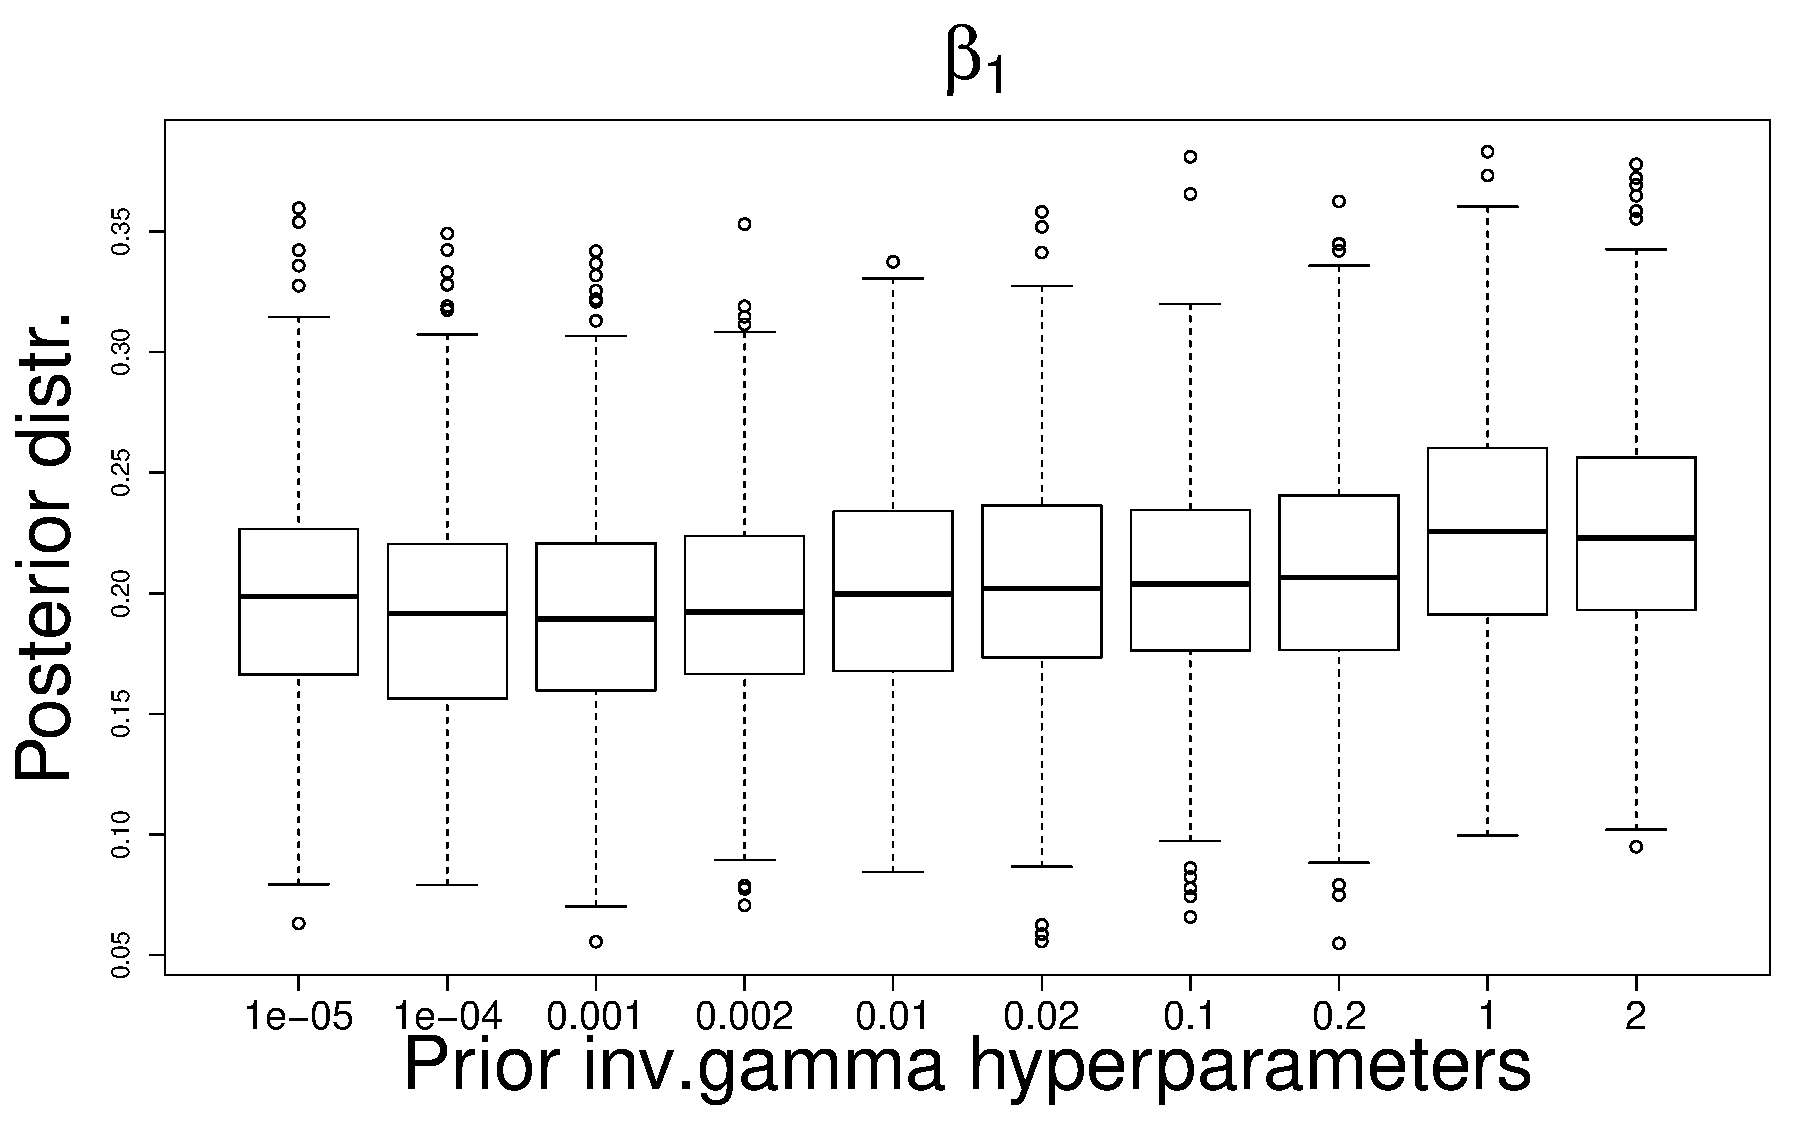
\includegraphics[scale=0.25]{Sensitivity/beta_1_sensitivity.pdf}~
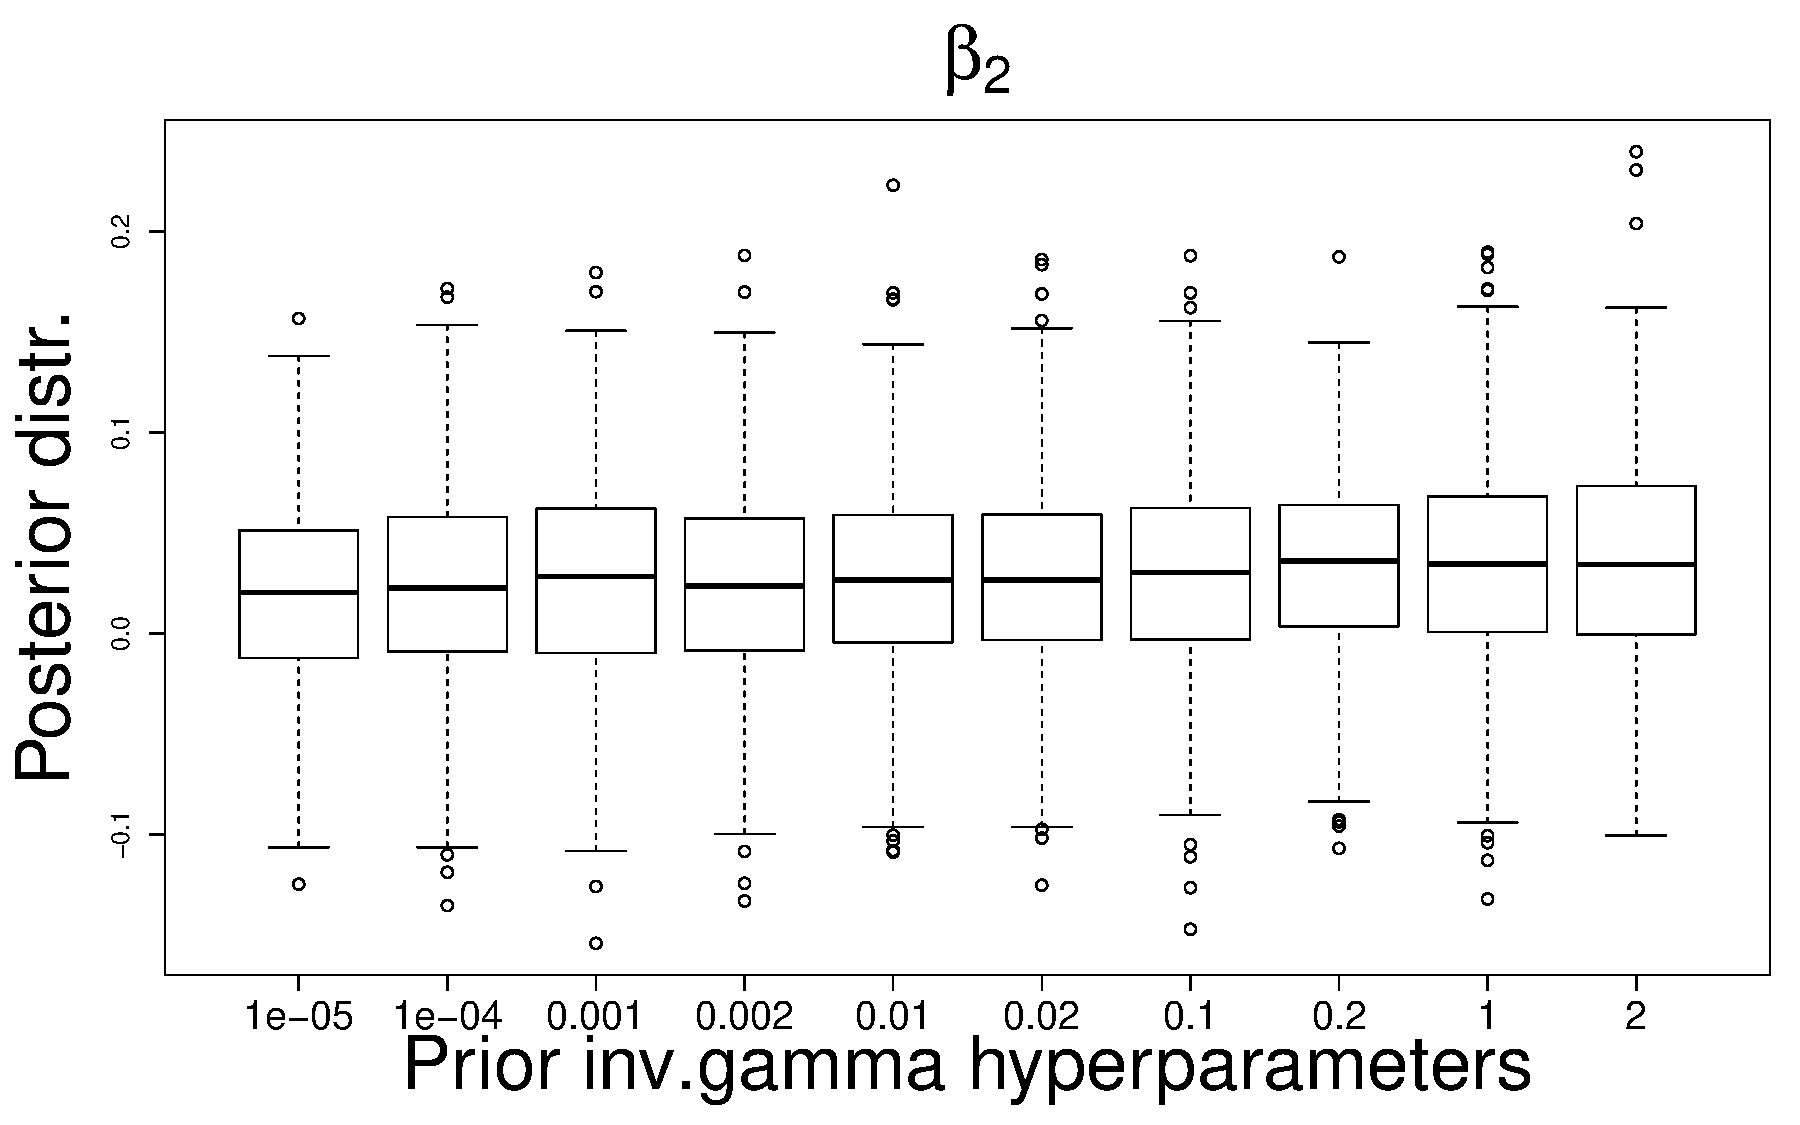
\includegraphics[scale=0.25]{Sensitivity/beta_2_sensitivity.pdf}\\
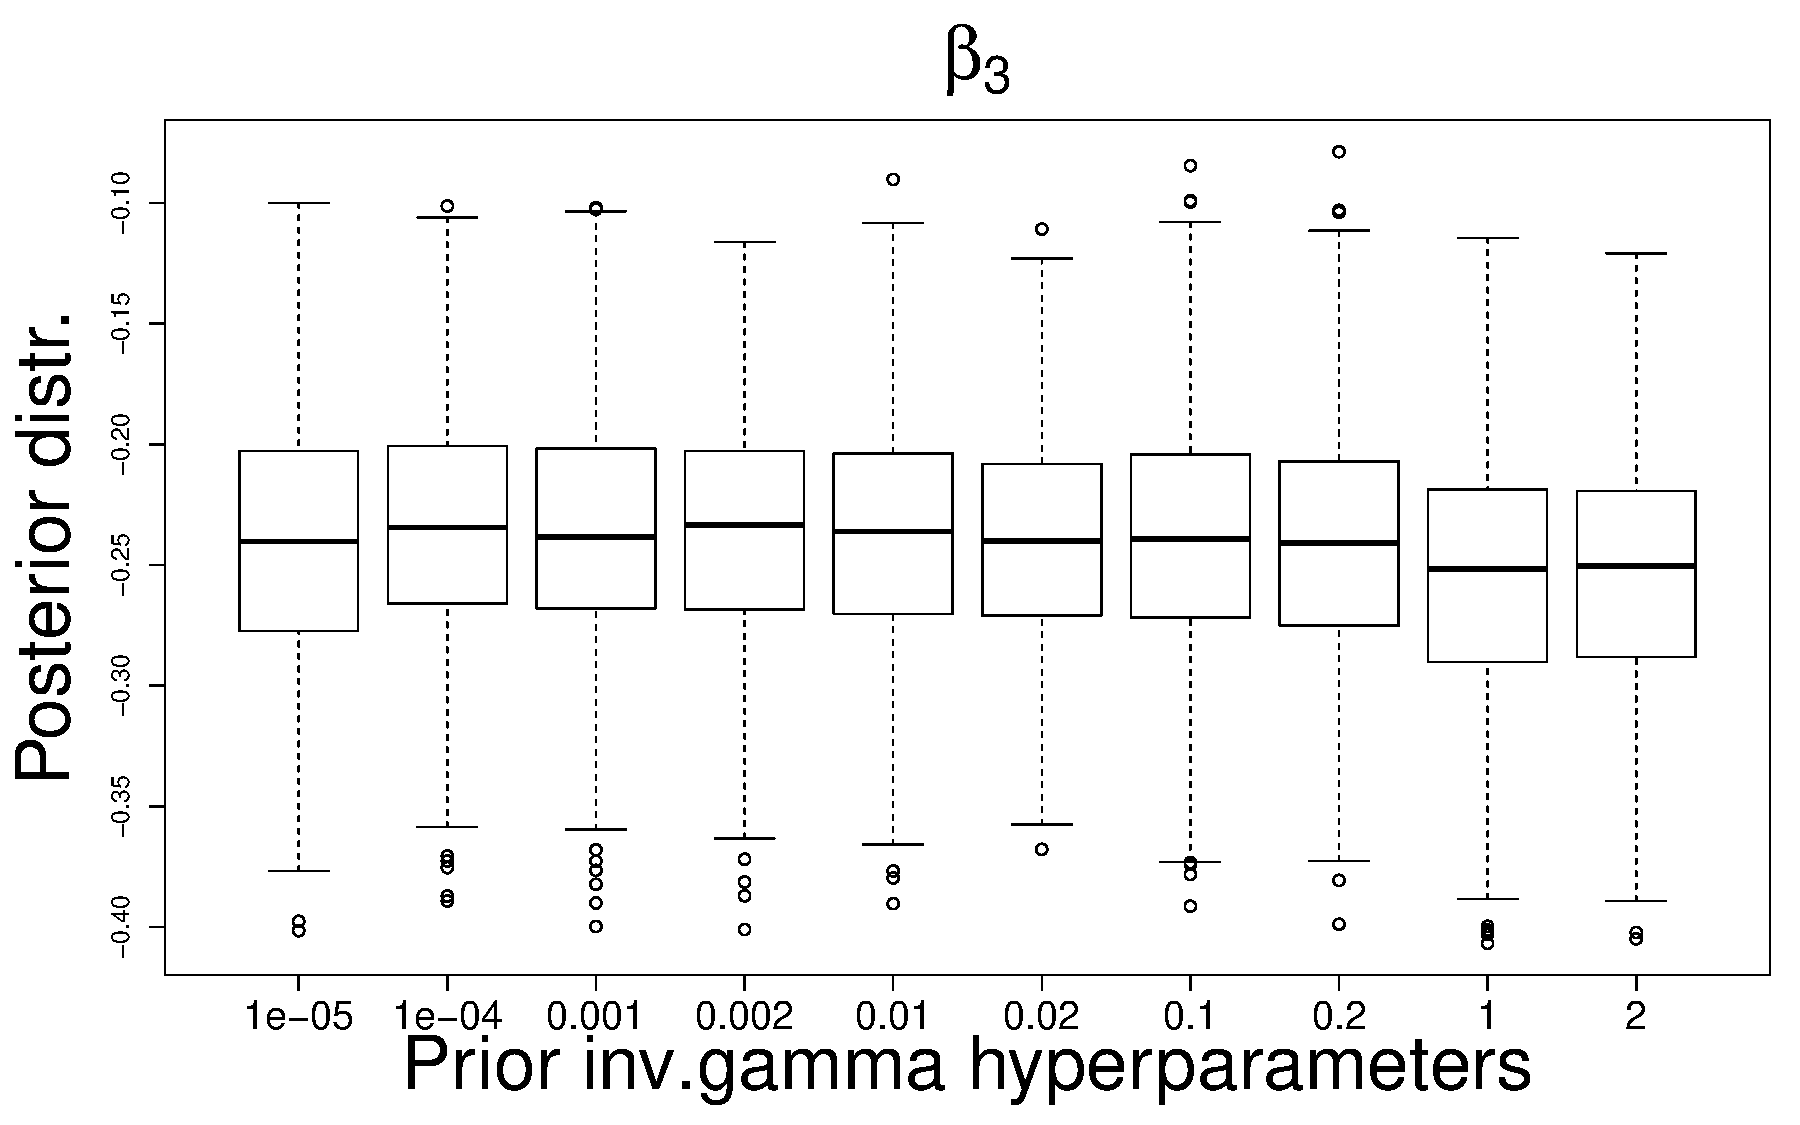
\includegraphics[scale=0.25]{Sensitivity/beta_3_sensitivity.pdf}~
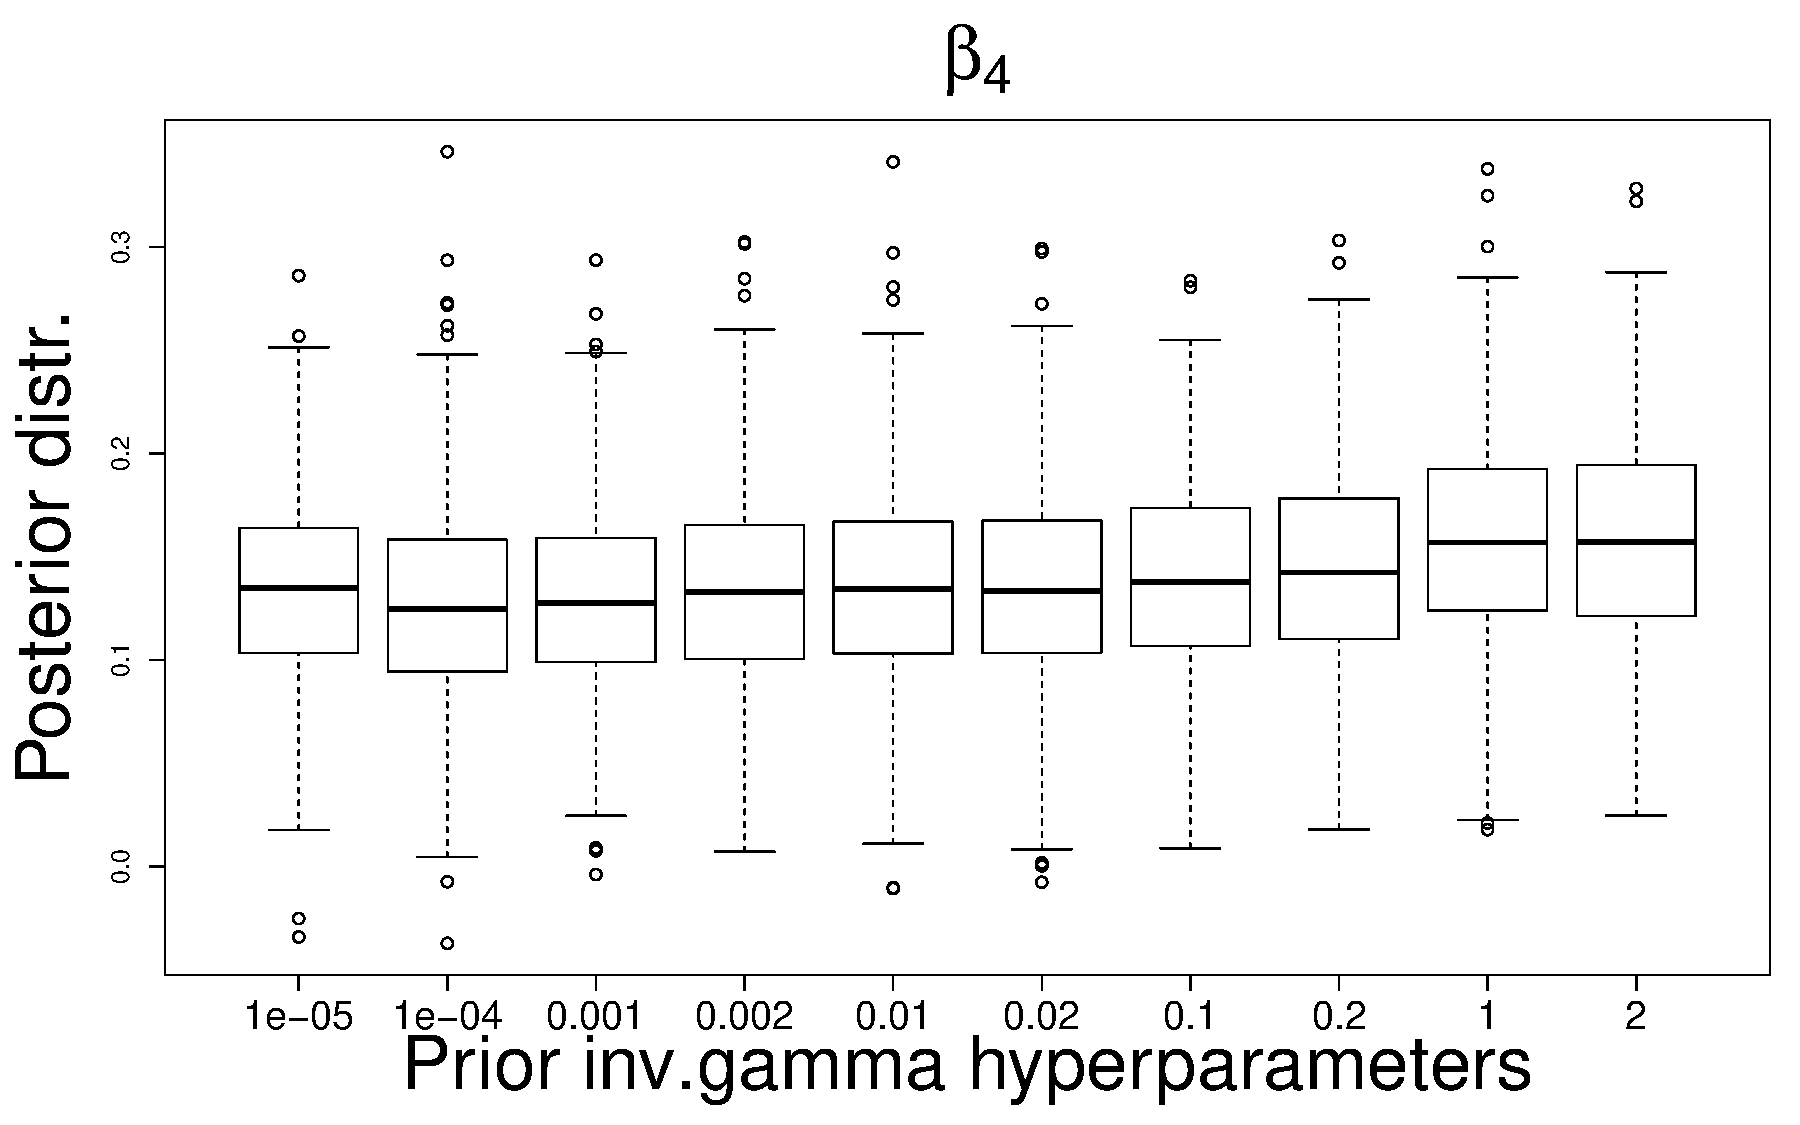
\includegraphics[scale=0.25]{Sensitivity/beta_4_sensitivity.pdf}\\
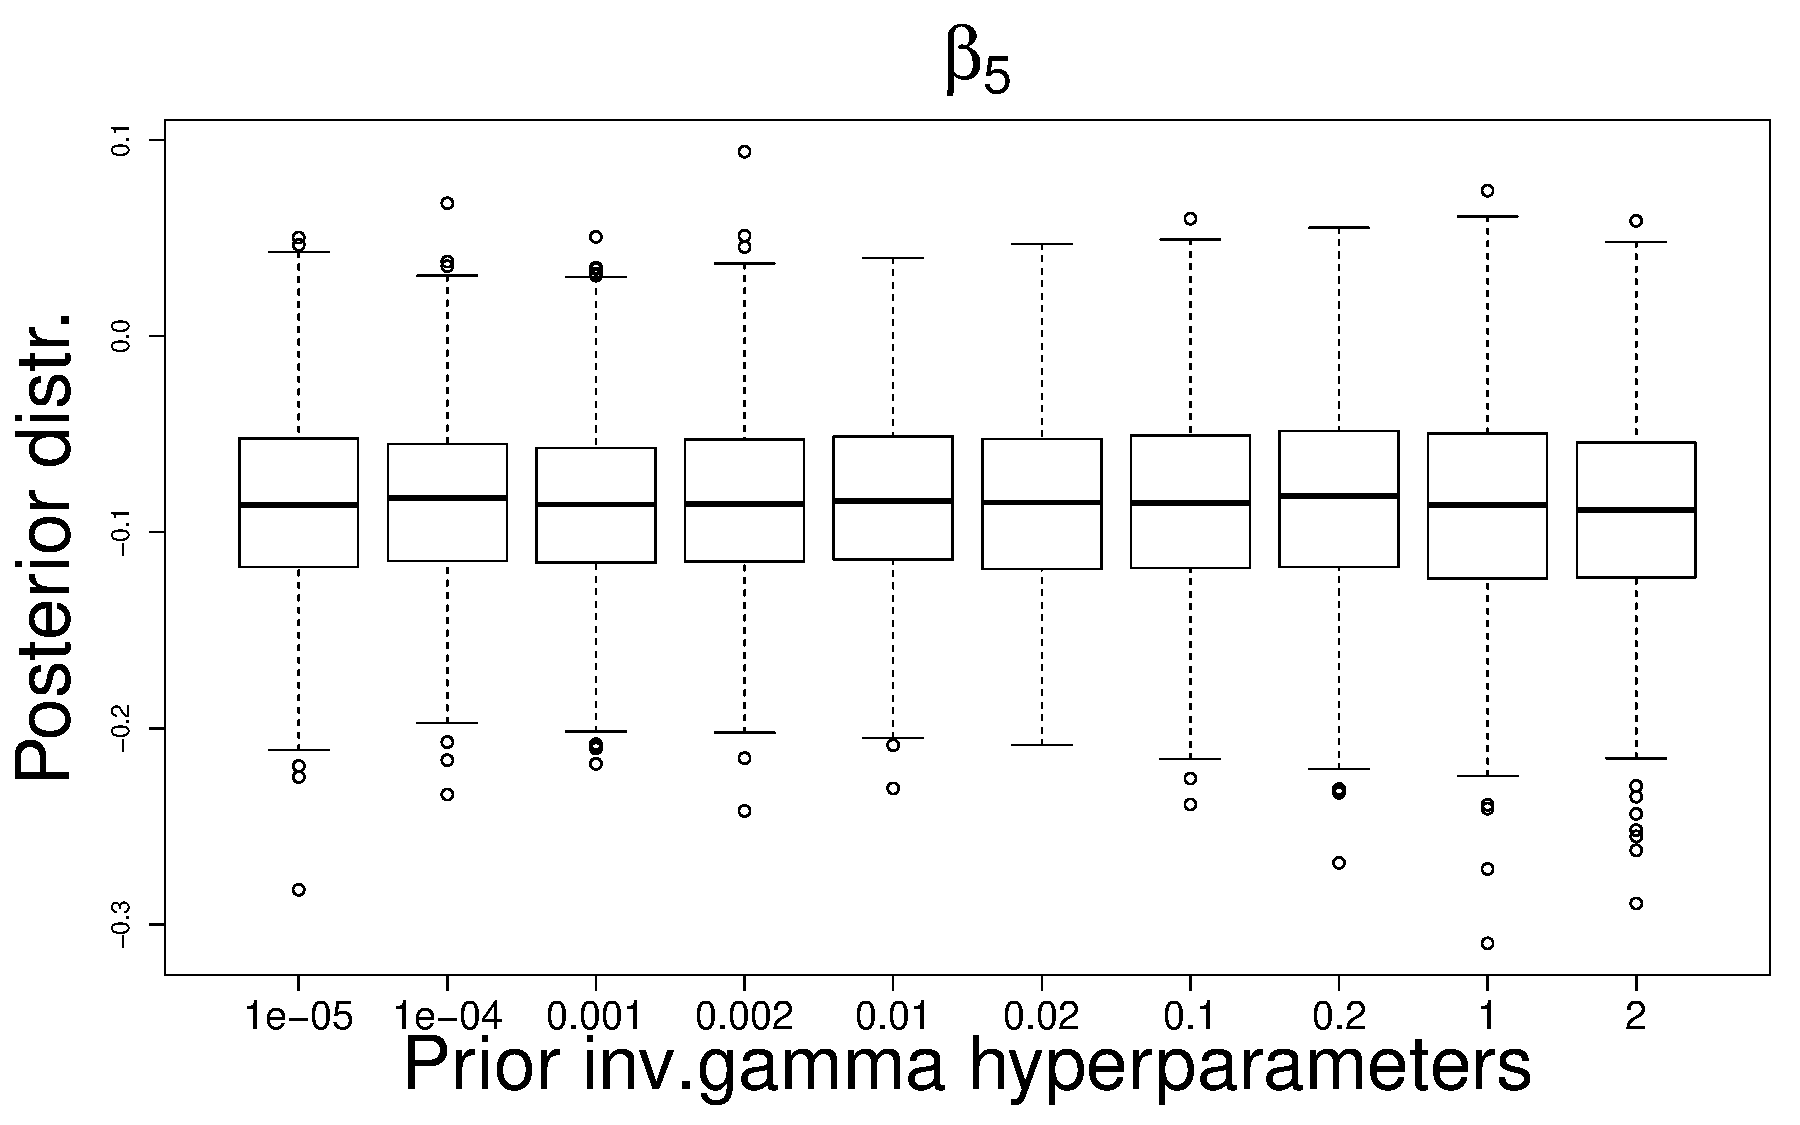
\includegraphics[scale=0.25]{Sensitivity/beta_5_sensitivity.pdf}~
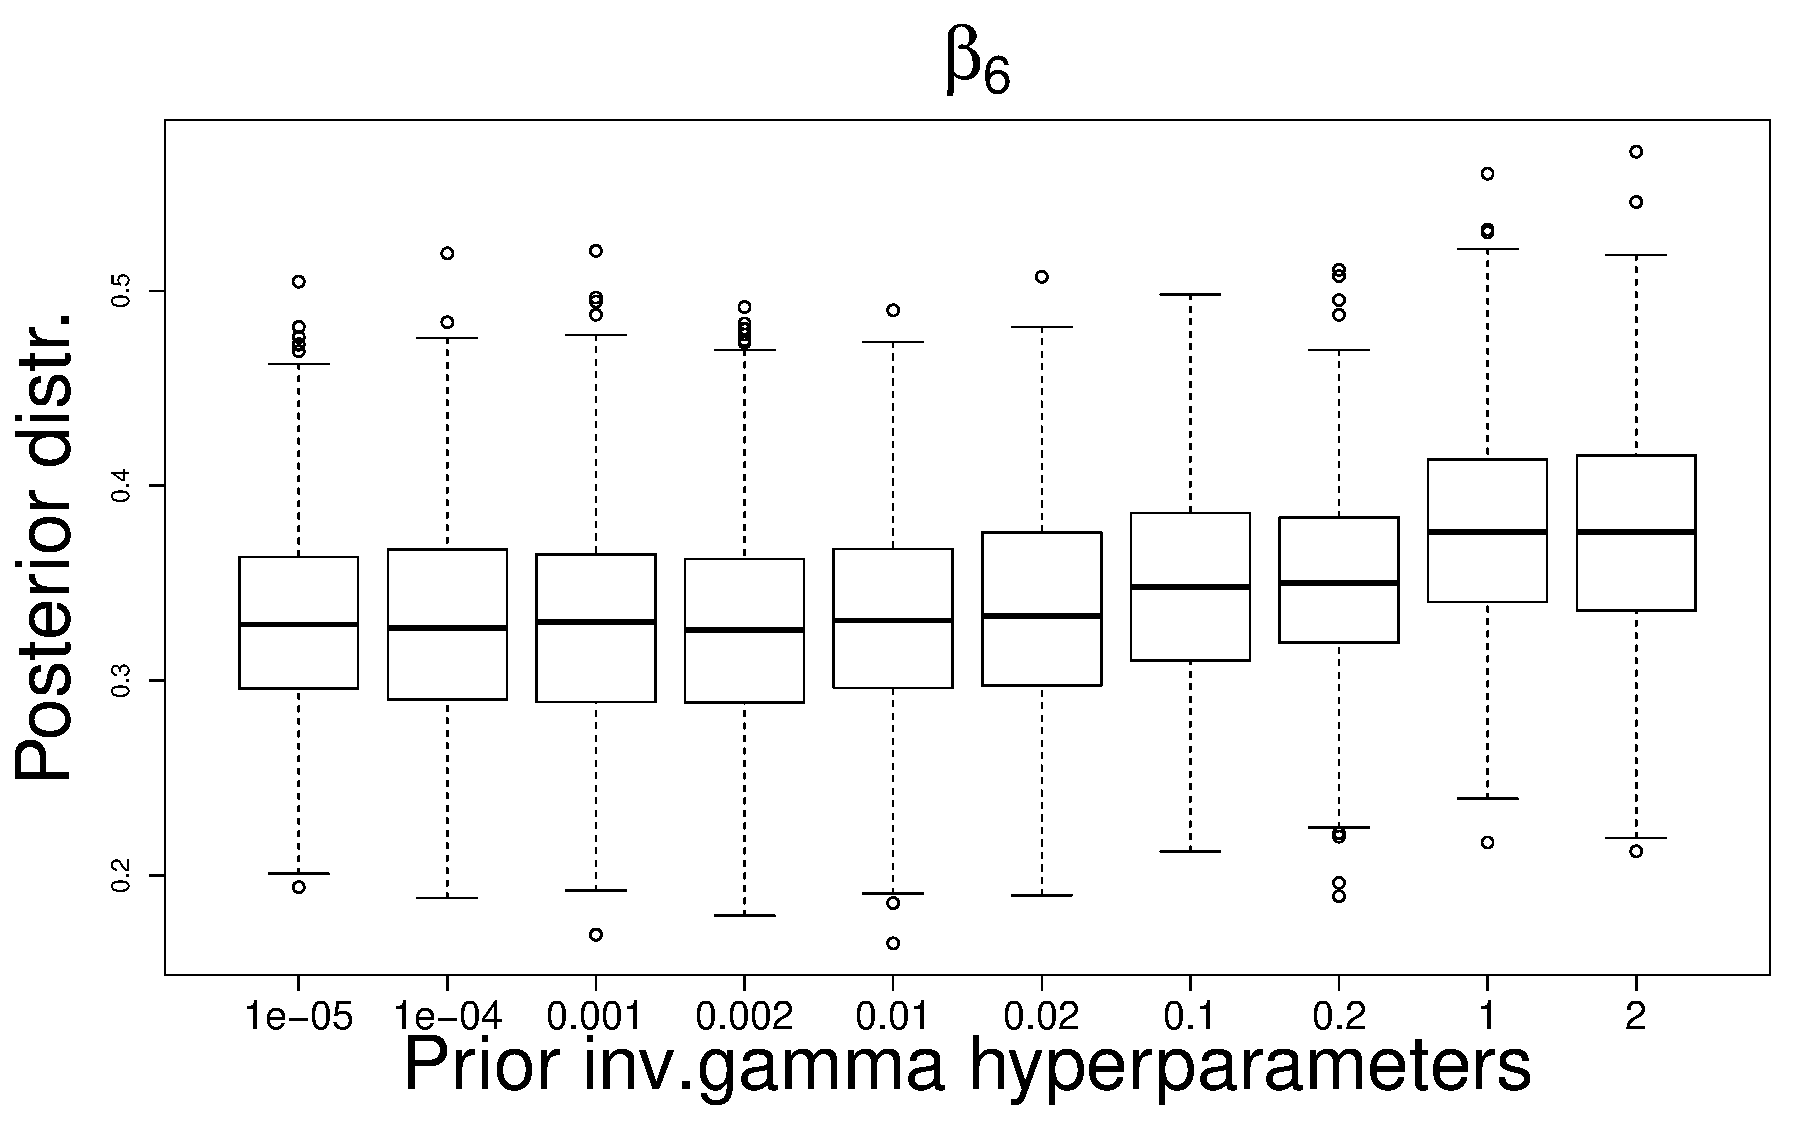
\includegraphics[scale=0.25]{Sensitivity/beta_6_sensitivity.pdf}\\
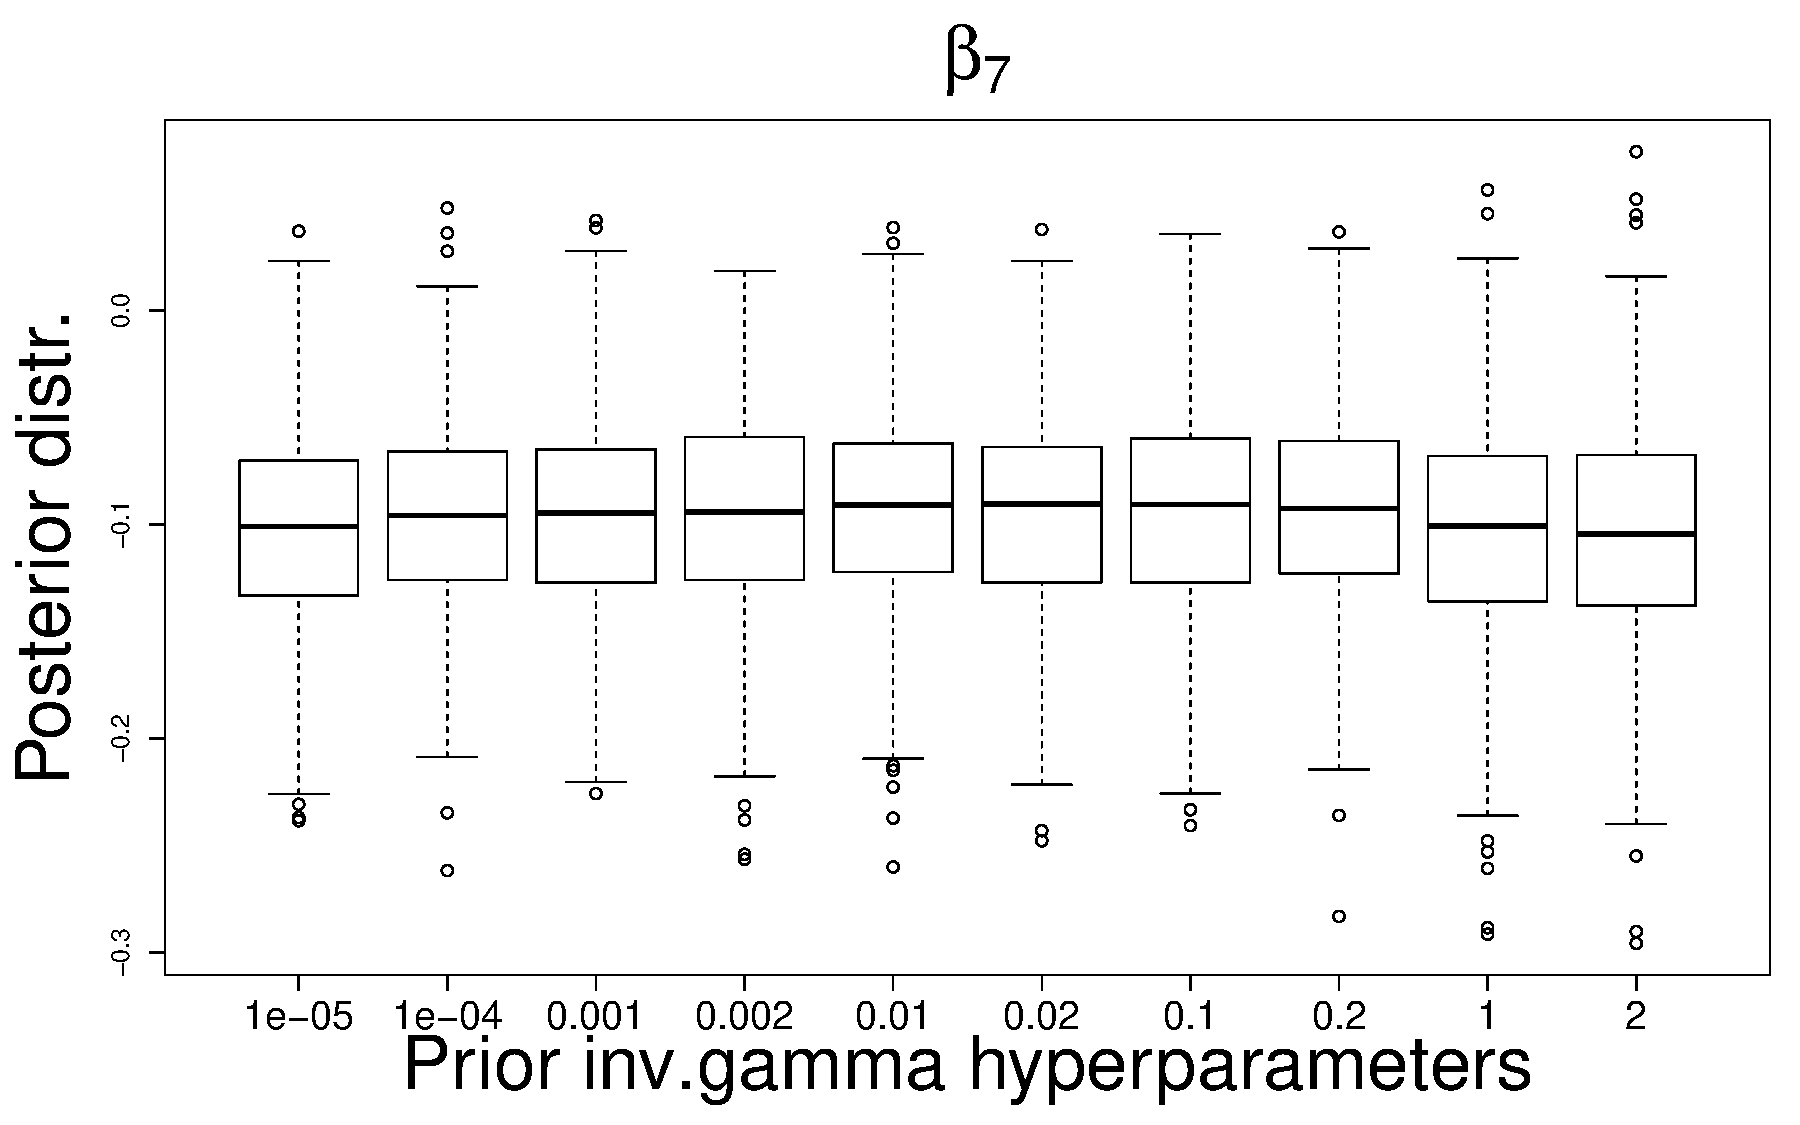
\includegraphics[scale=0.25]{Sensitivity/beta_7_sensitivity.pdf}~
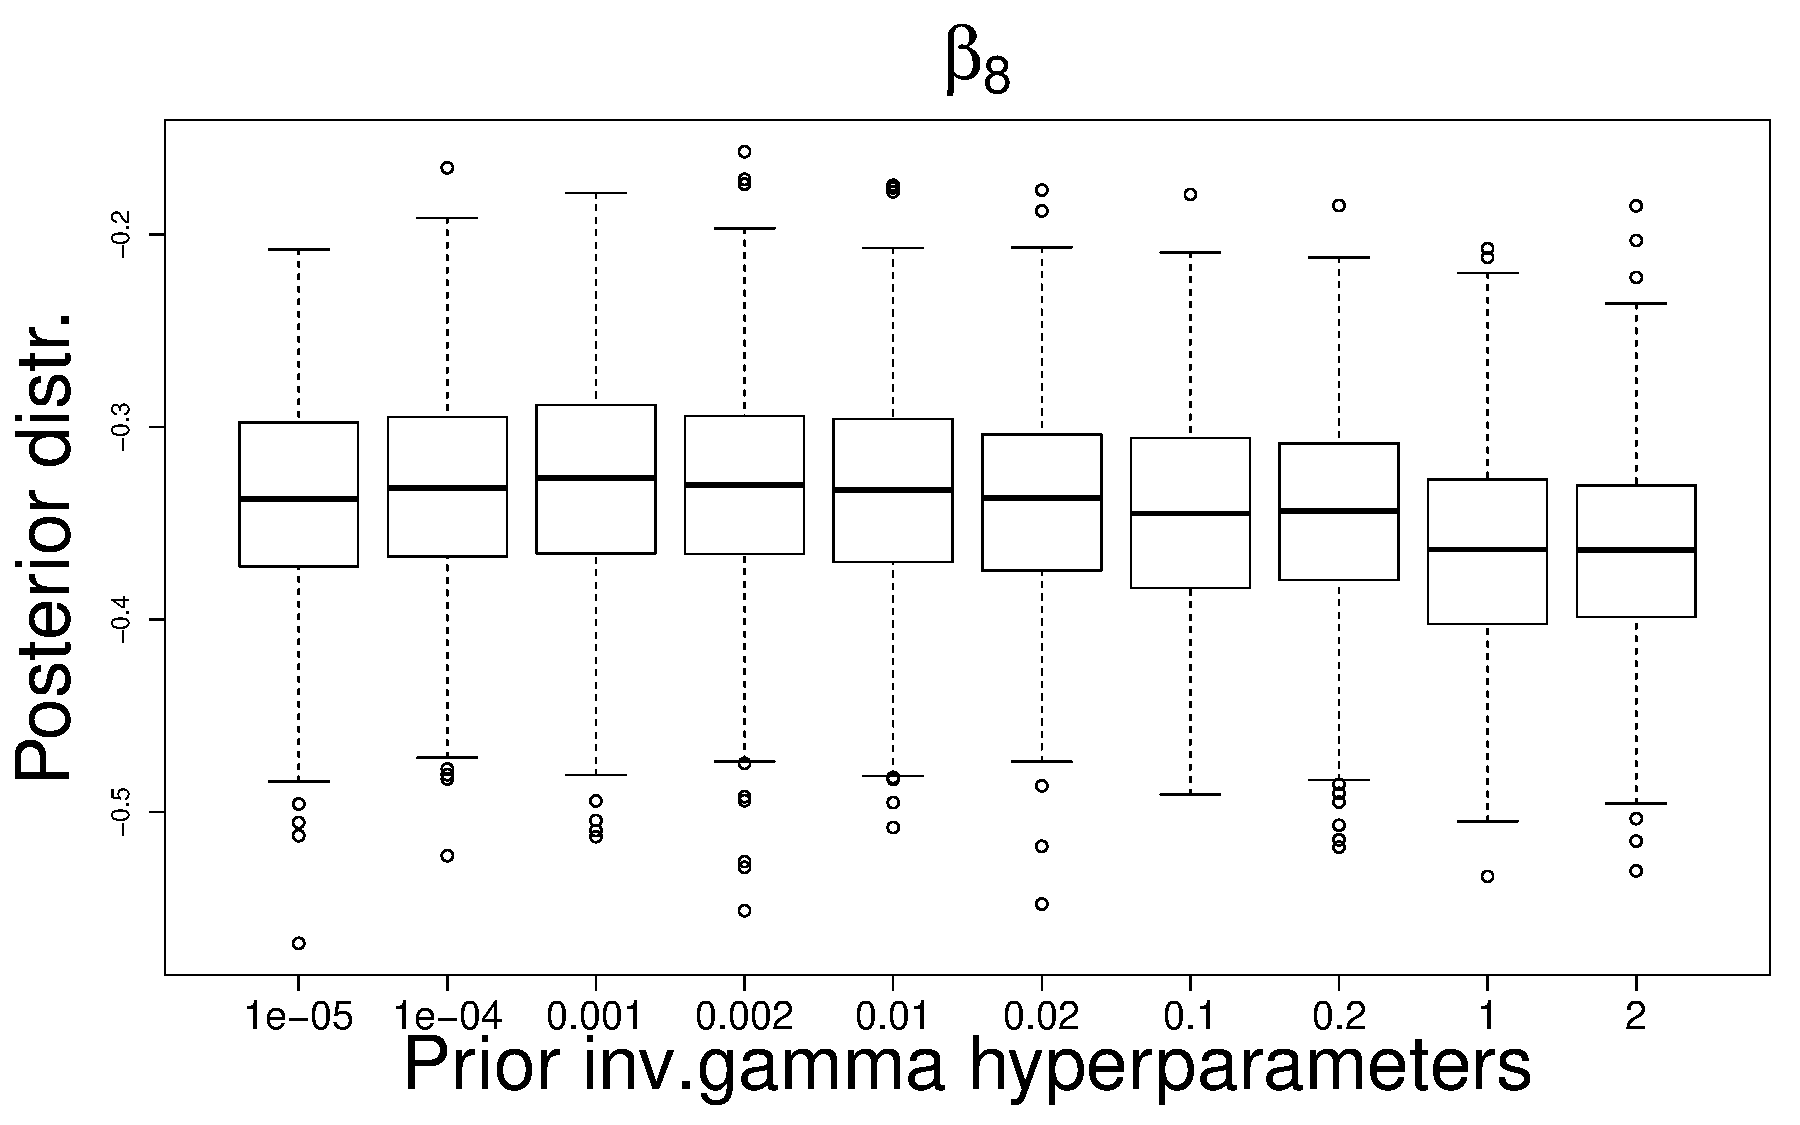
\includegraphics[scale=0.25]{Sensitivity/beta_8_sensitivity.pdf}\\
\caption{Sensitivity tests for the marginal posterior distributions of the point abilities parameters $\beta_1, \ldots,\beta_8$ by varying the hyperparameters of the inverse-gamma prior assigned to $\tau^2_{\beta}$. {\tt rjags}, 1000 MCMC iterations, burn-in period of 100 iterations.}
\label{figS3}
\end{figure}

\begin{figure}
\centering

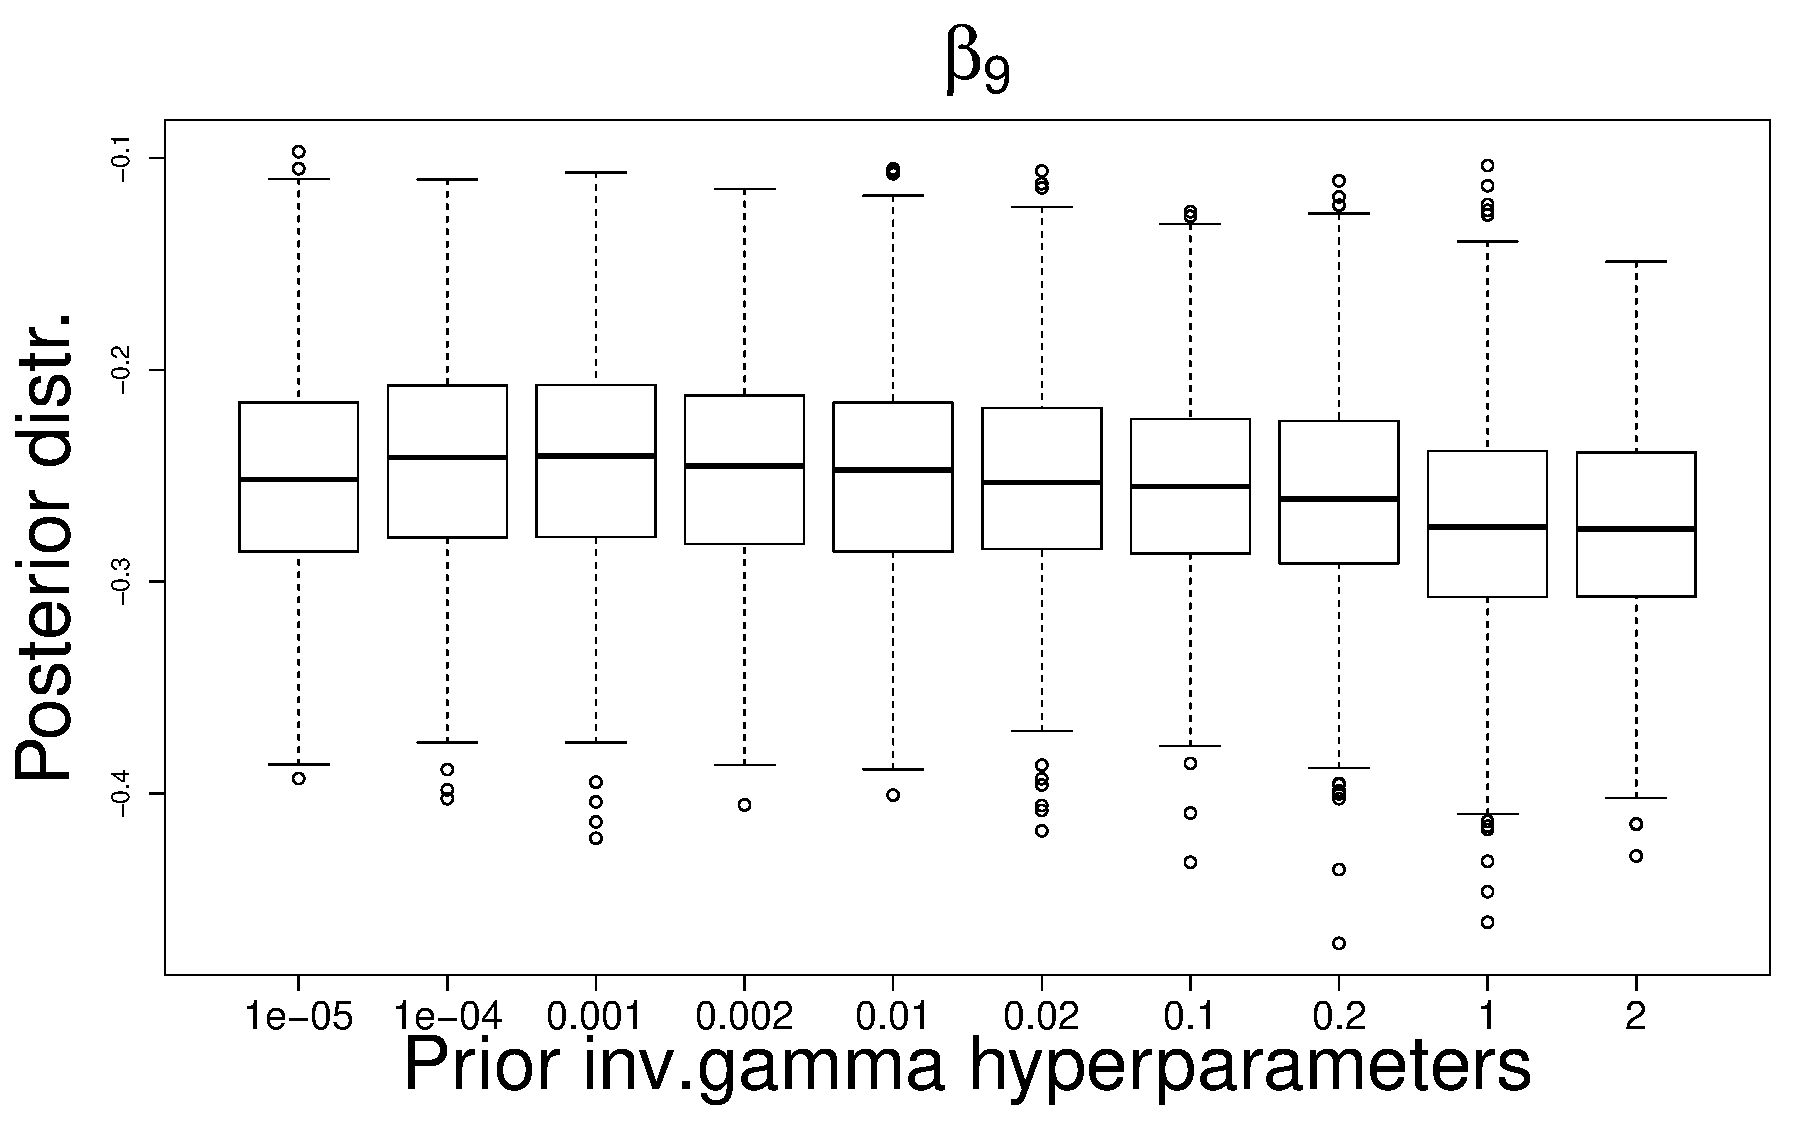
\includegraphics[scale=0.25]{Sensitivity/beta_9_sensitivity.pdf}~
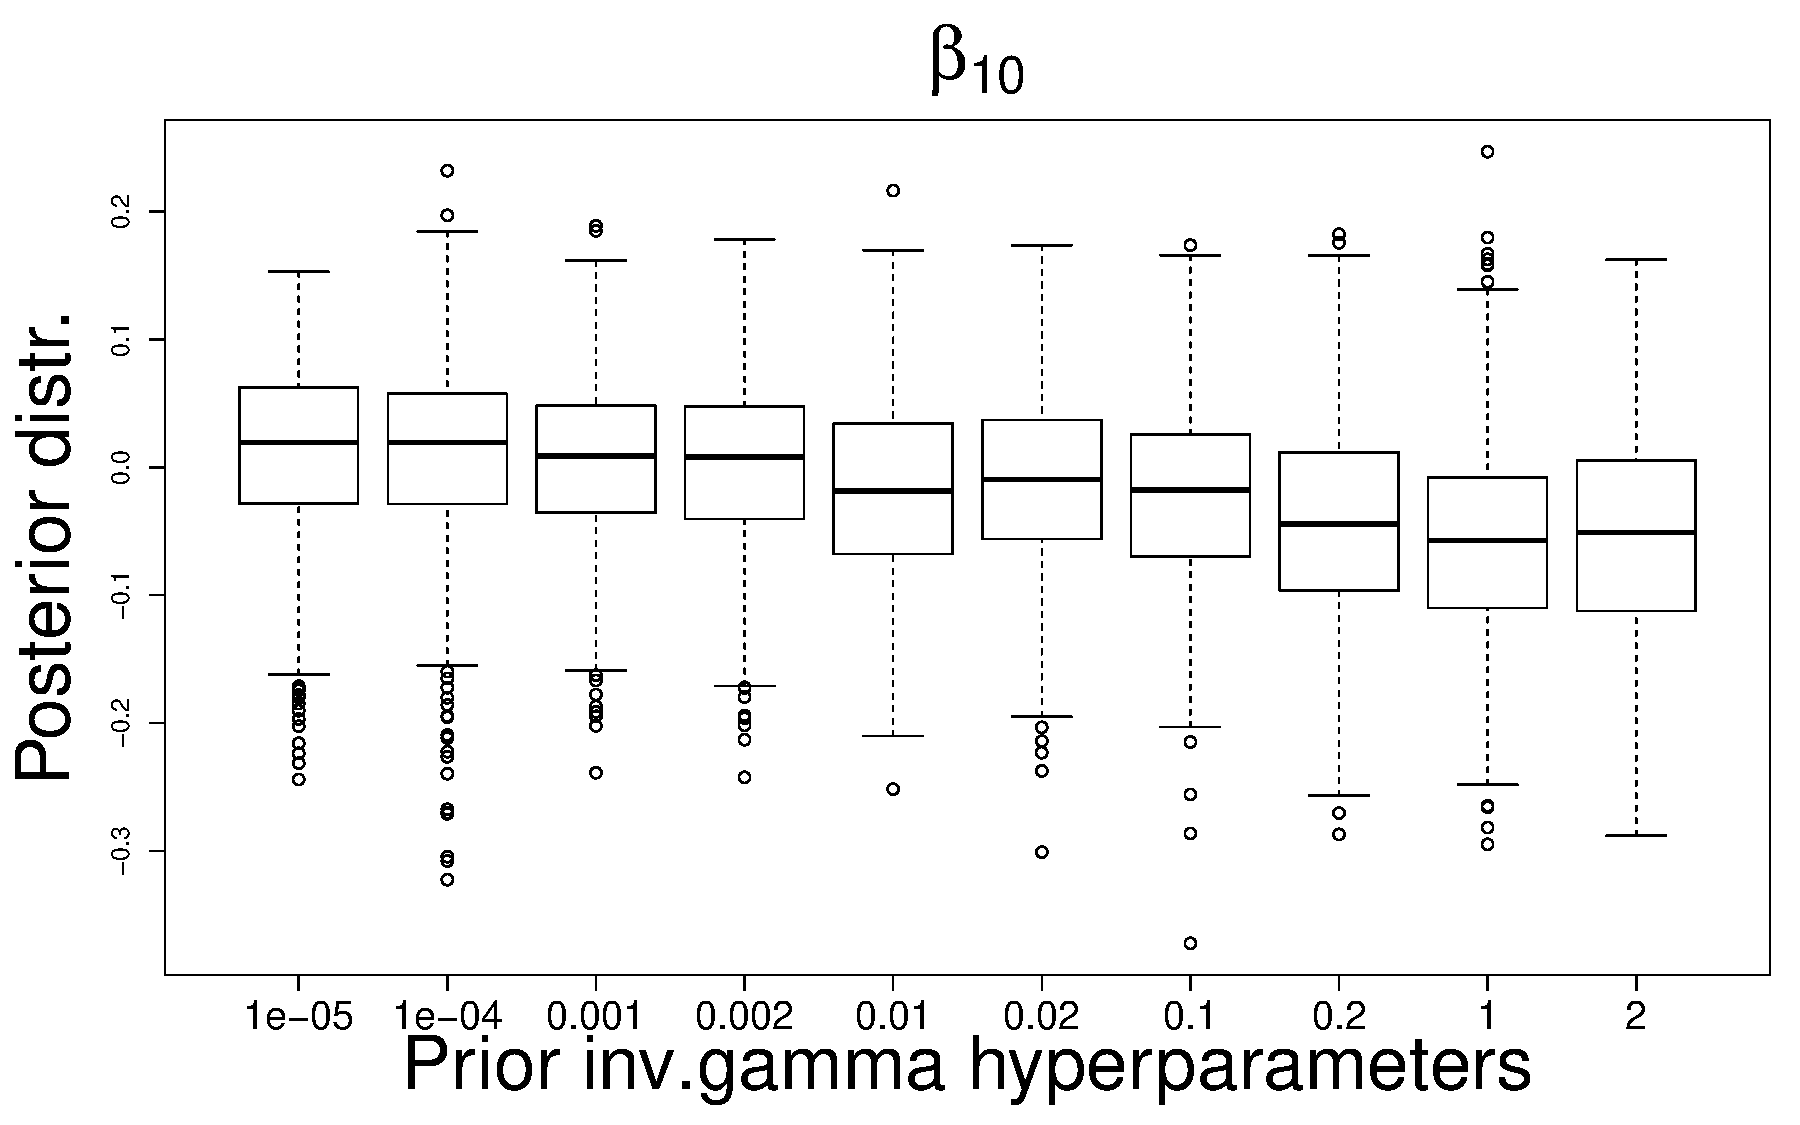
\includegraphics[scale=0.25]{Sensitivity/beta_10_sensitivity.pdf}\\
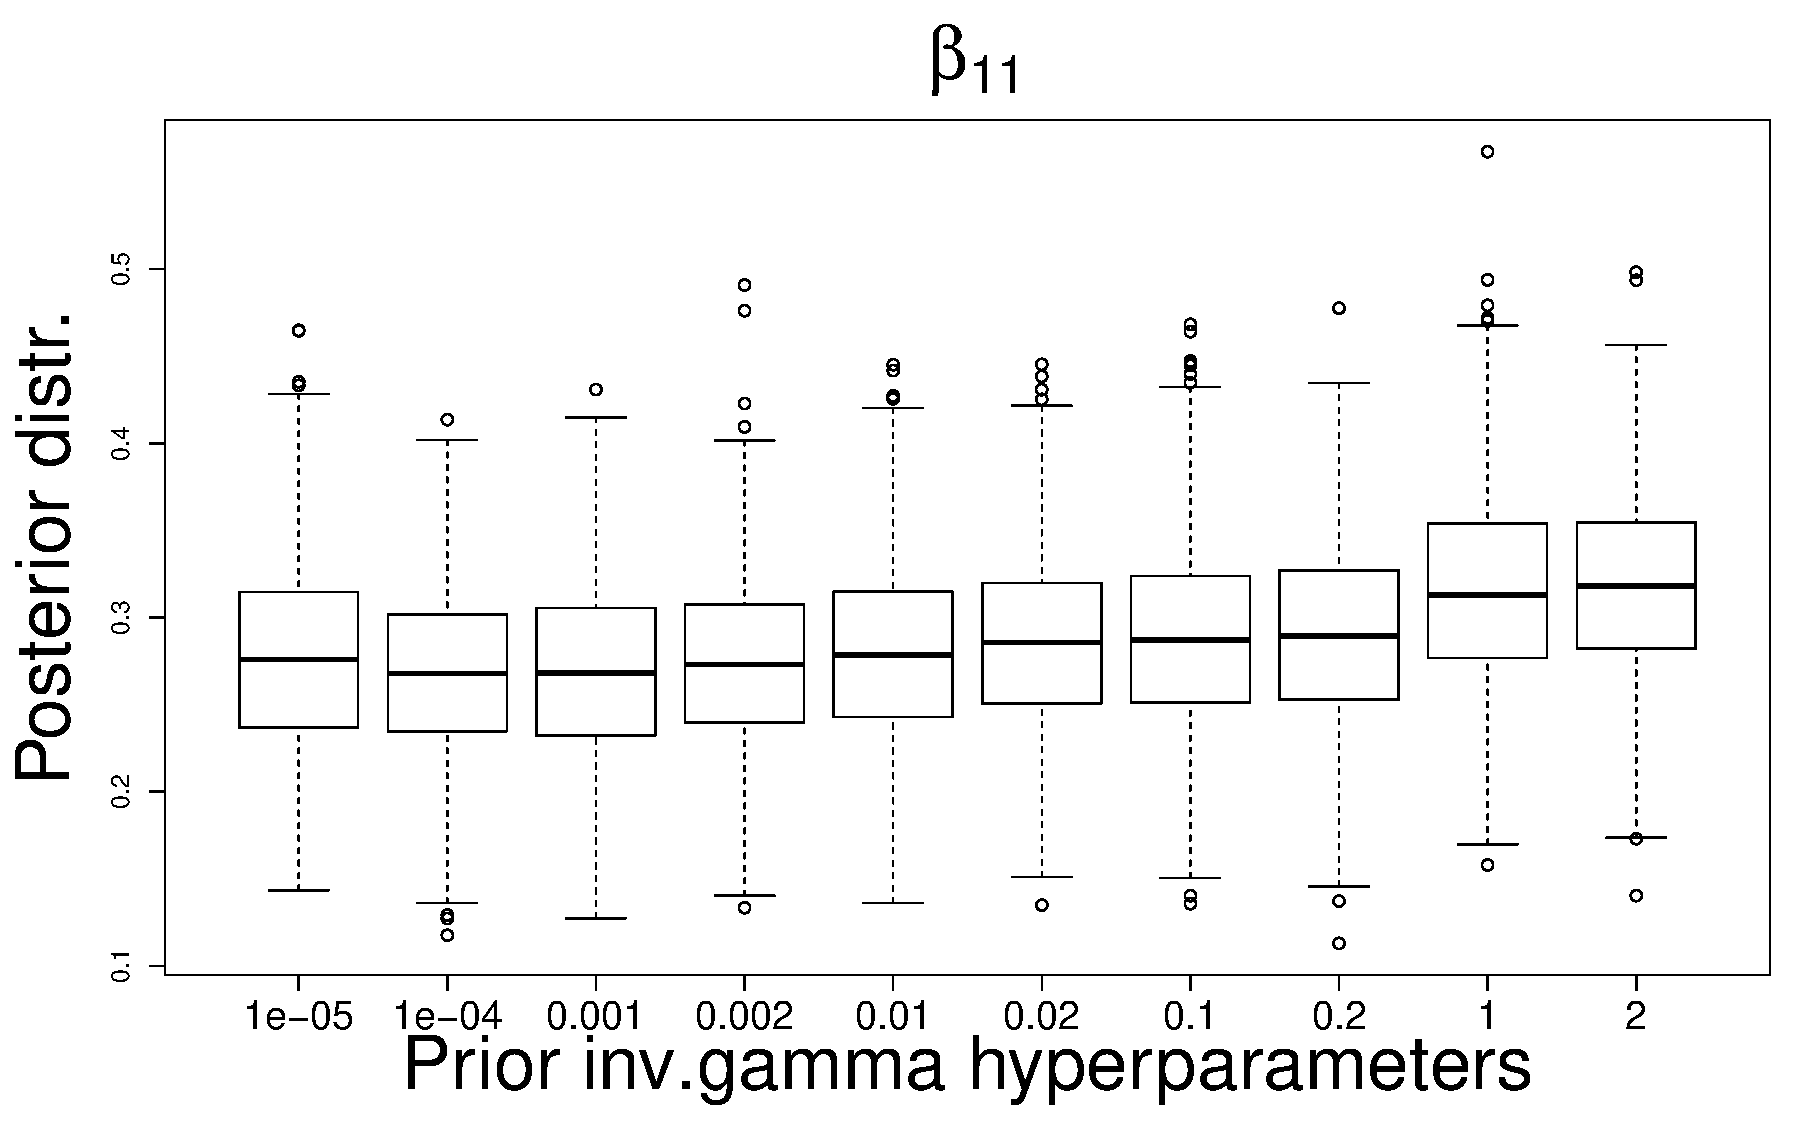
\includegraphics[scale=0.25]{Sensitivity/beta_11_sensitivity.pdf}~
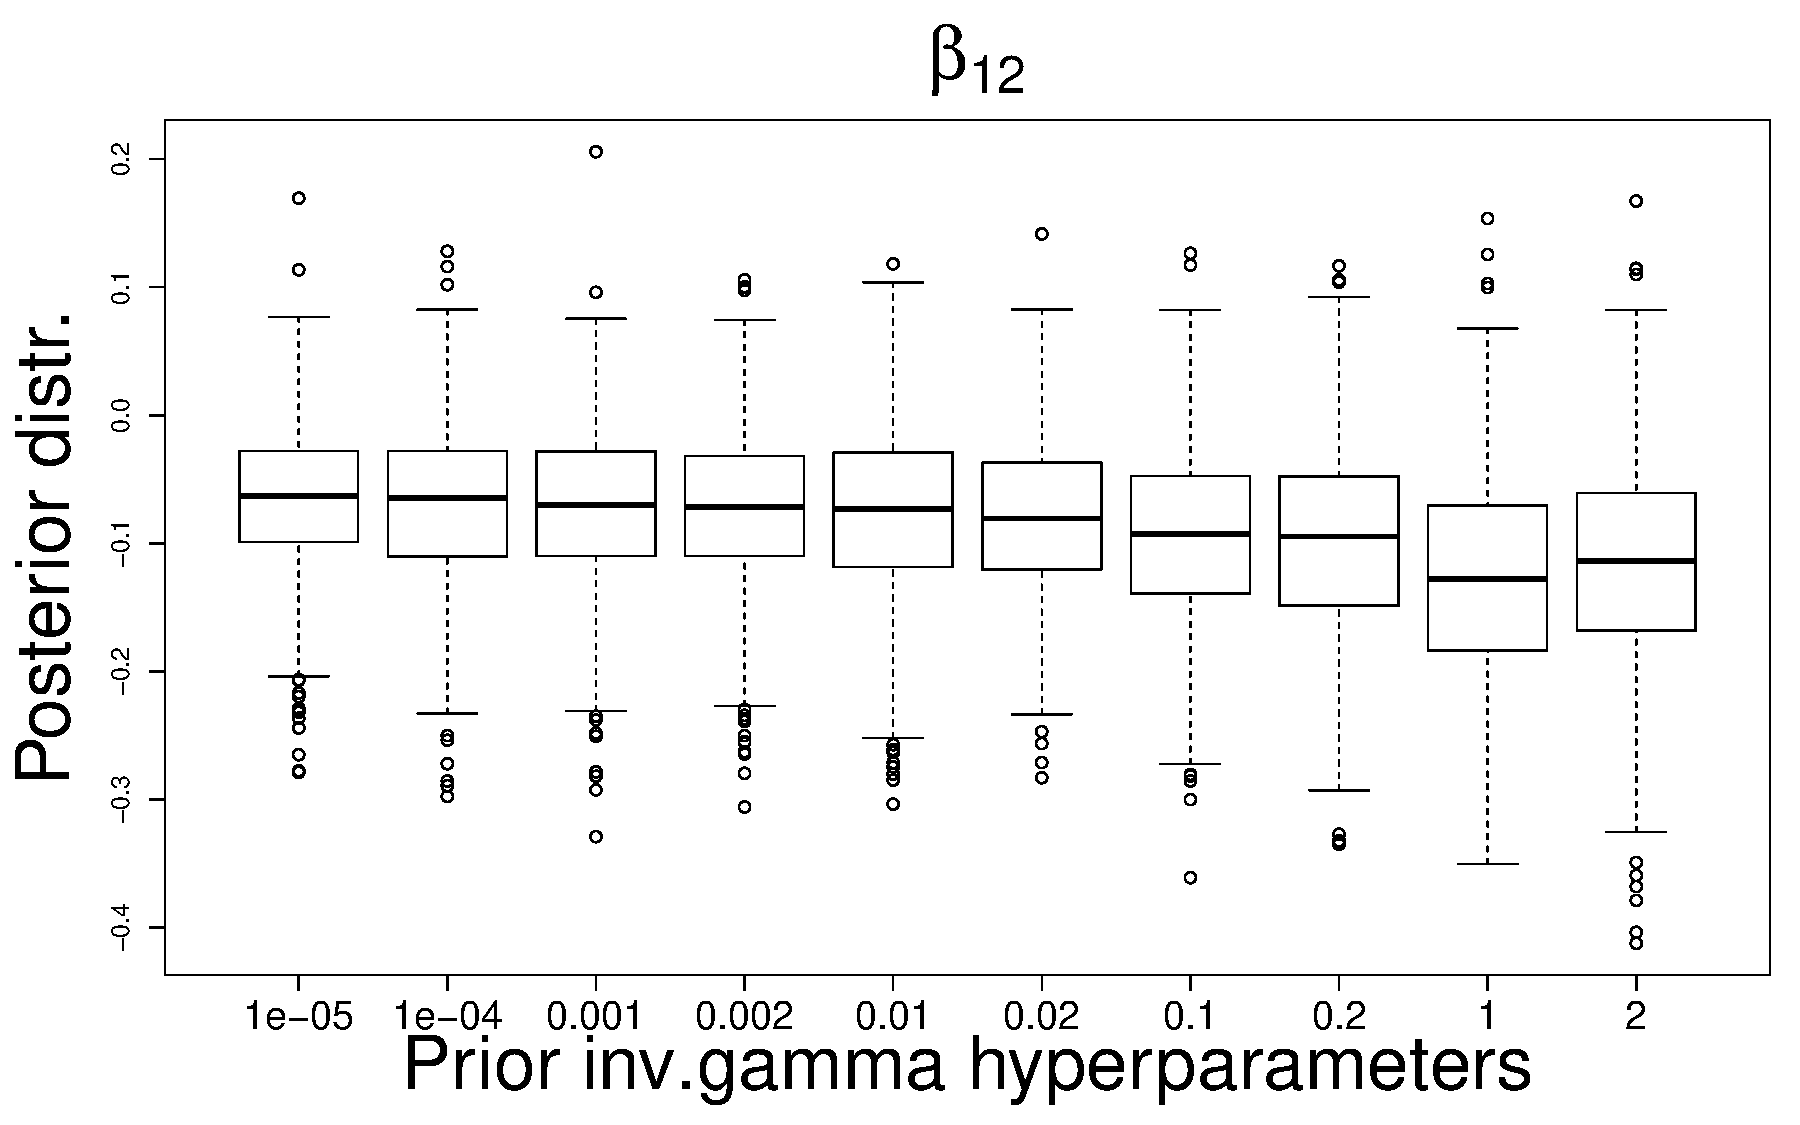
\includegraphics[scale=0.25]{Sensitivity/beta_12_sensitivity.pdf}\\
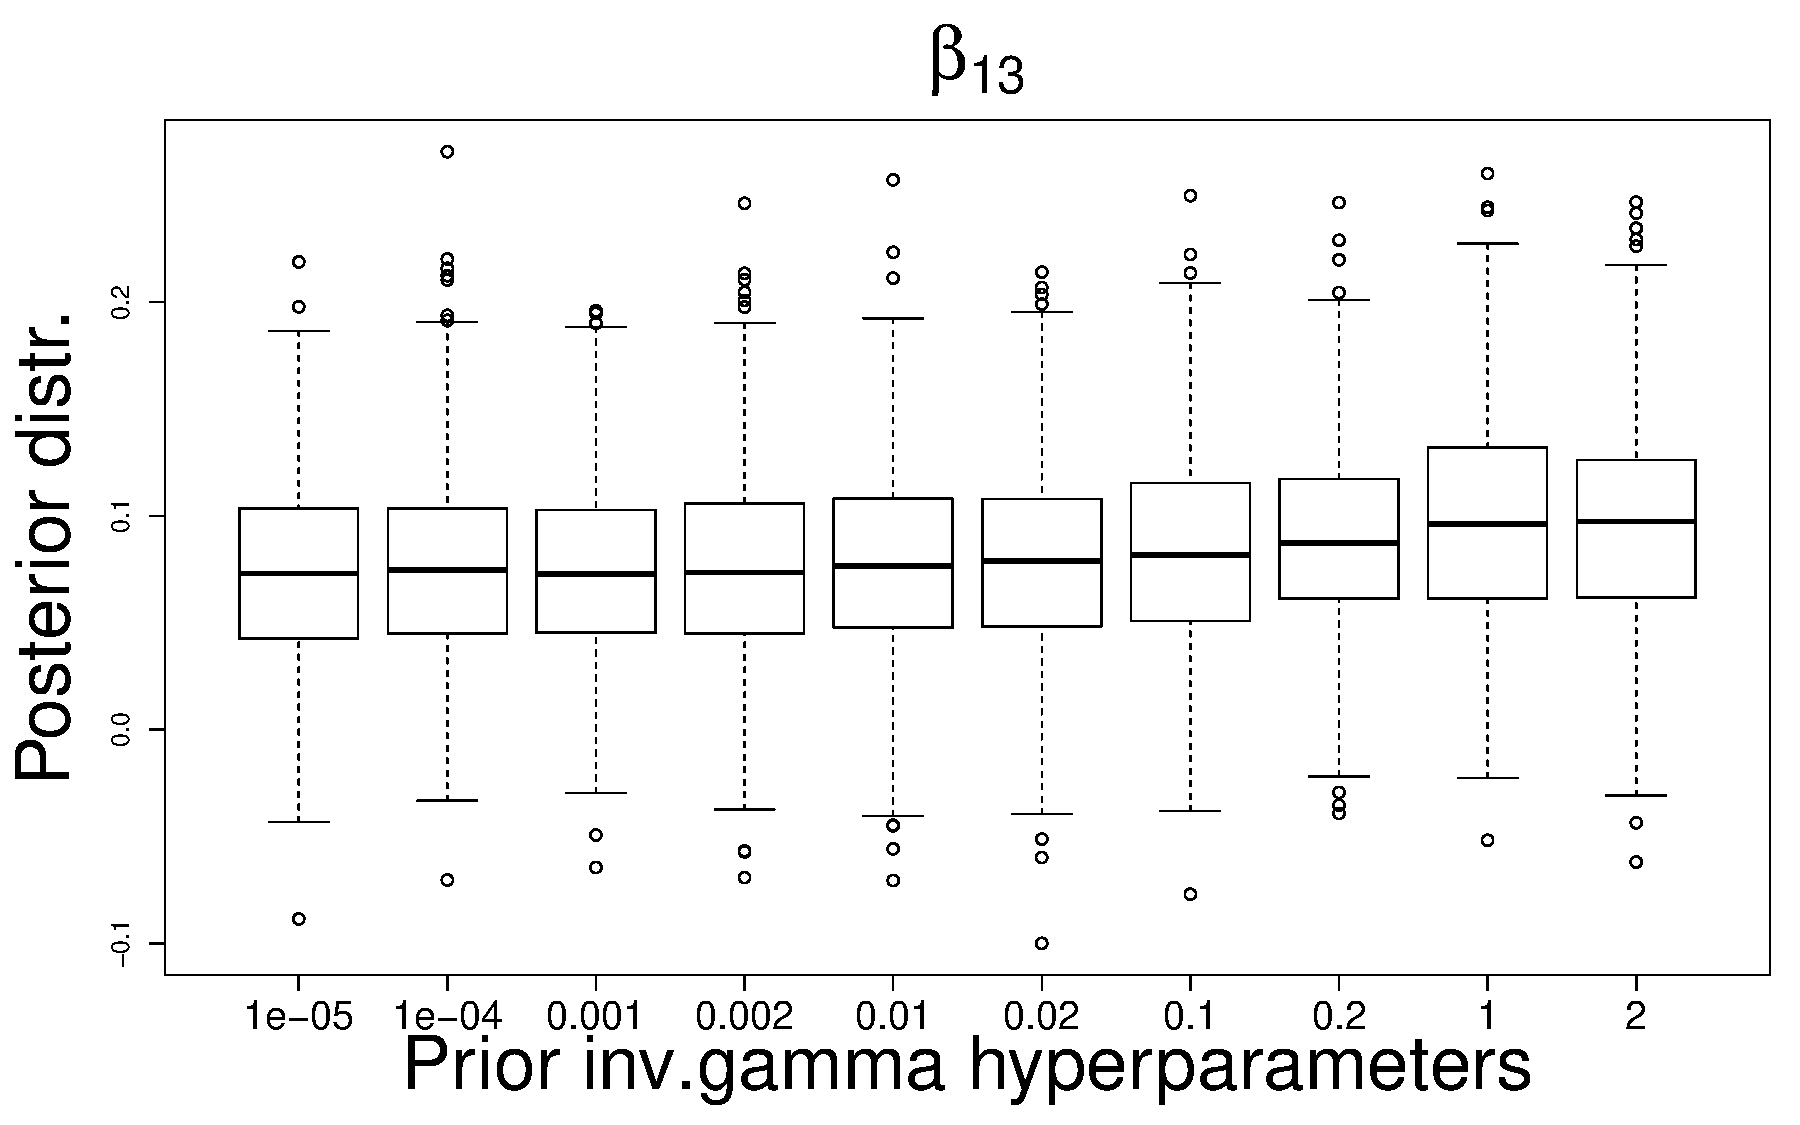
\includegraphics[scale=0.25]{Sensitivity/beta_13_sensitivity.pdf}~
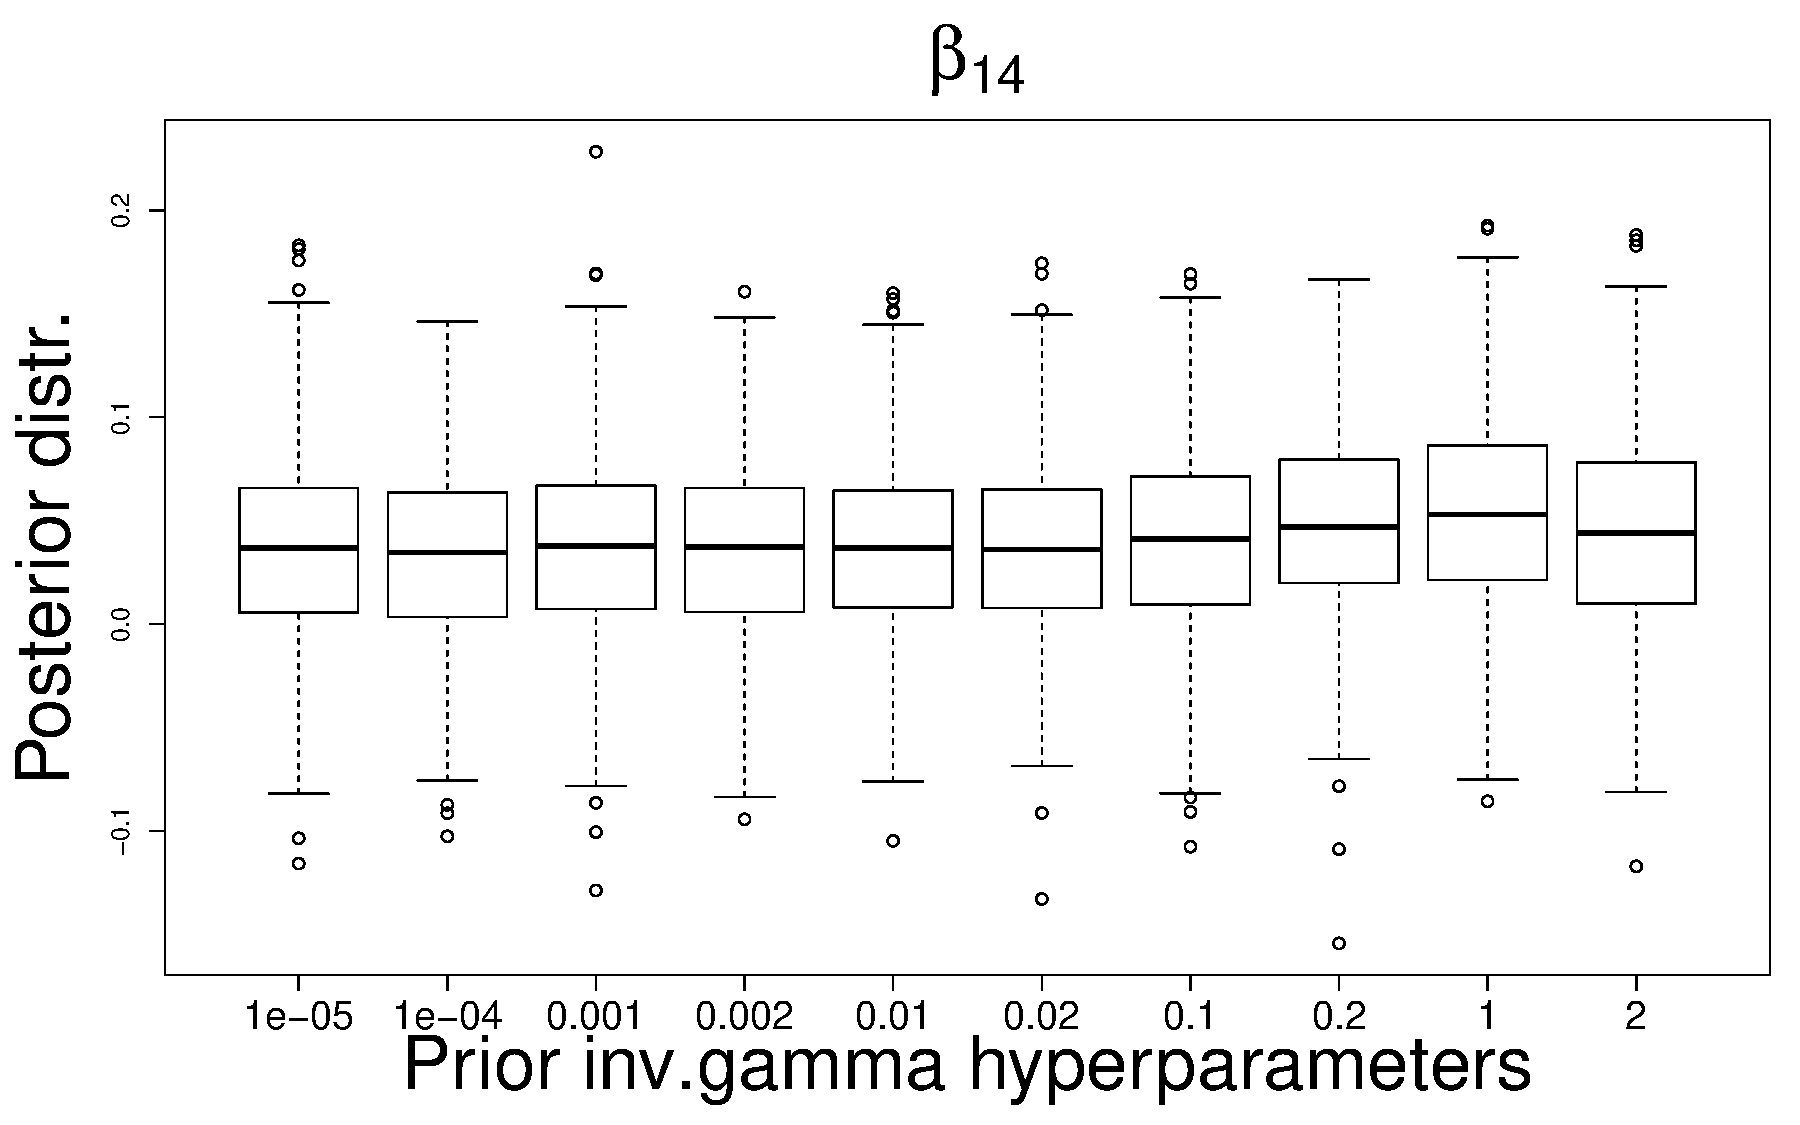
\includegraphics[scale=0.25]{Sensitivity/beta_14_sensitivity.pdf}\\
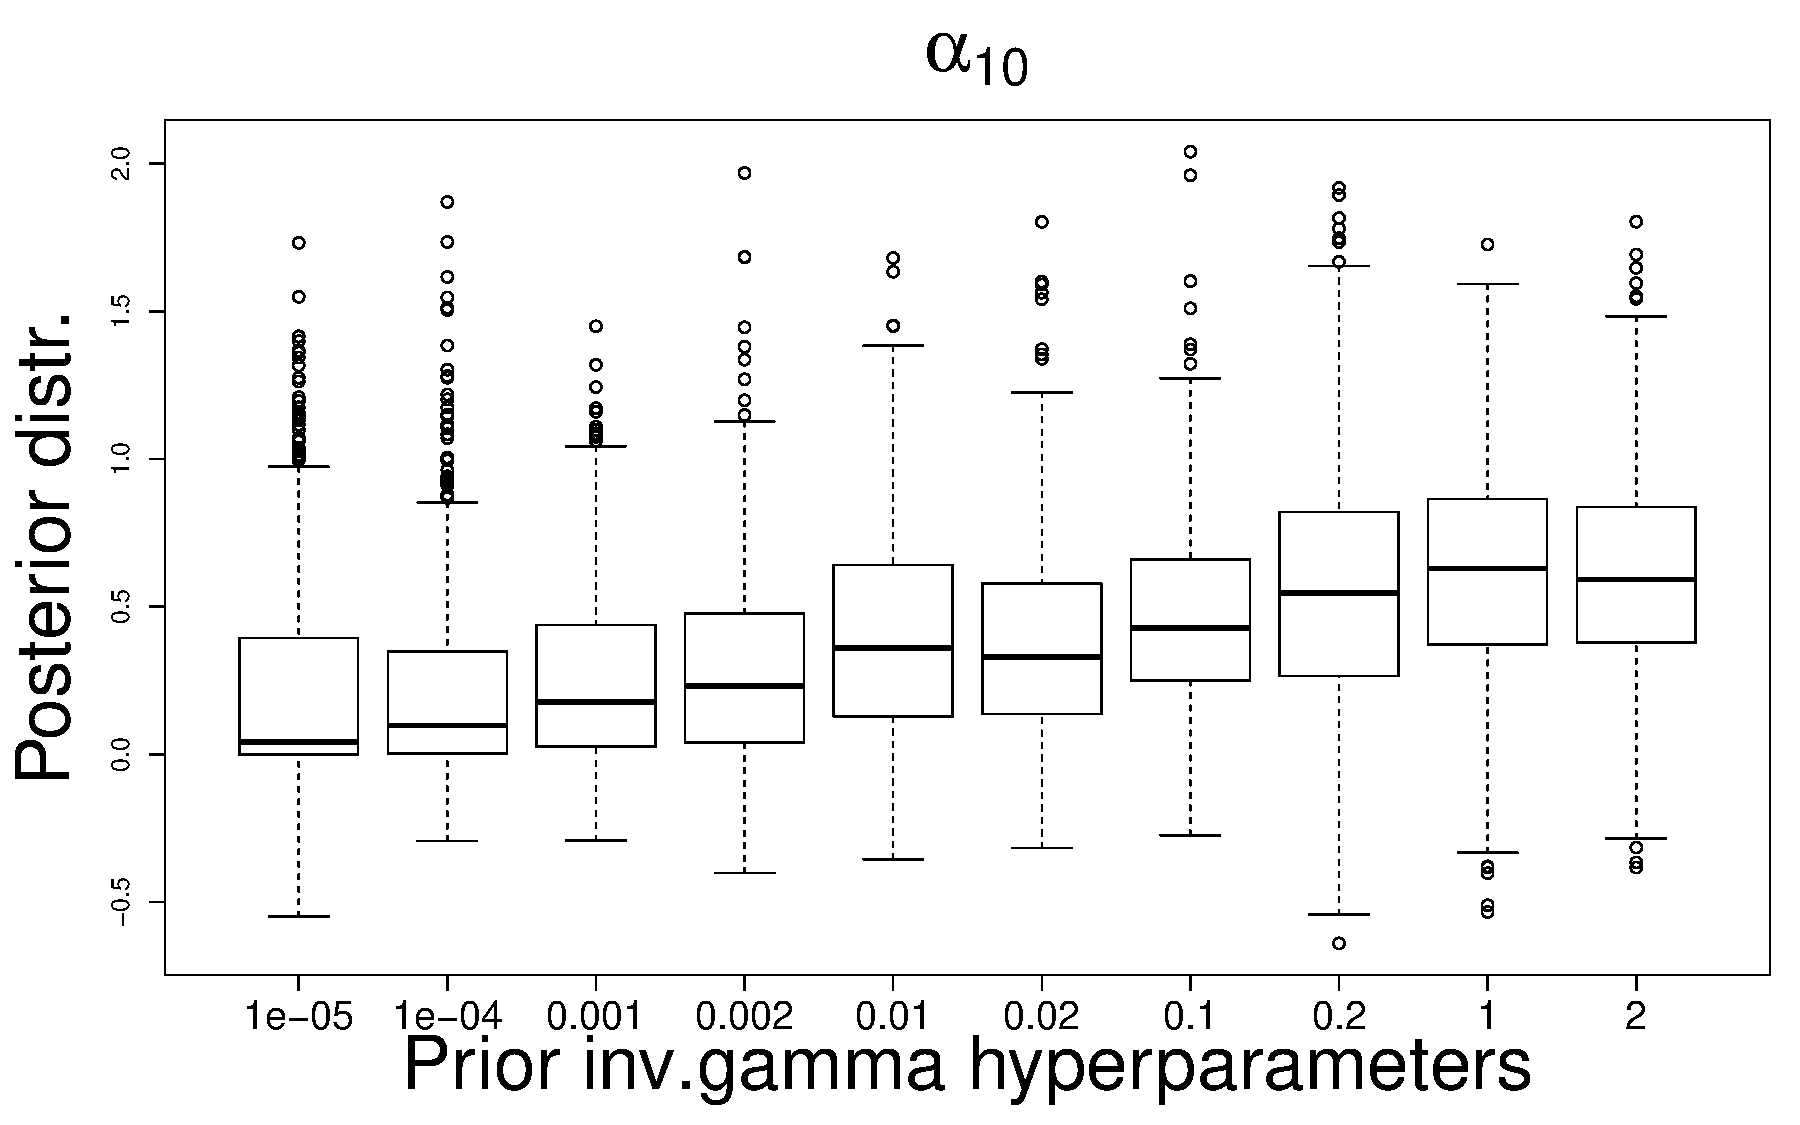
\includegraphics[scale=0.25]{Sensitivity/alpha_10_sensitivity.pdf}~
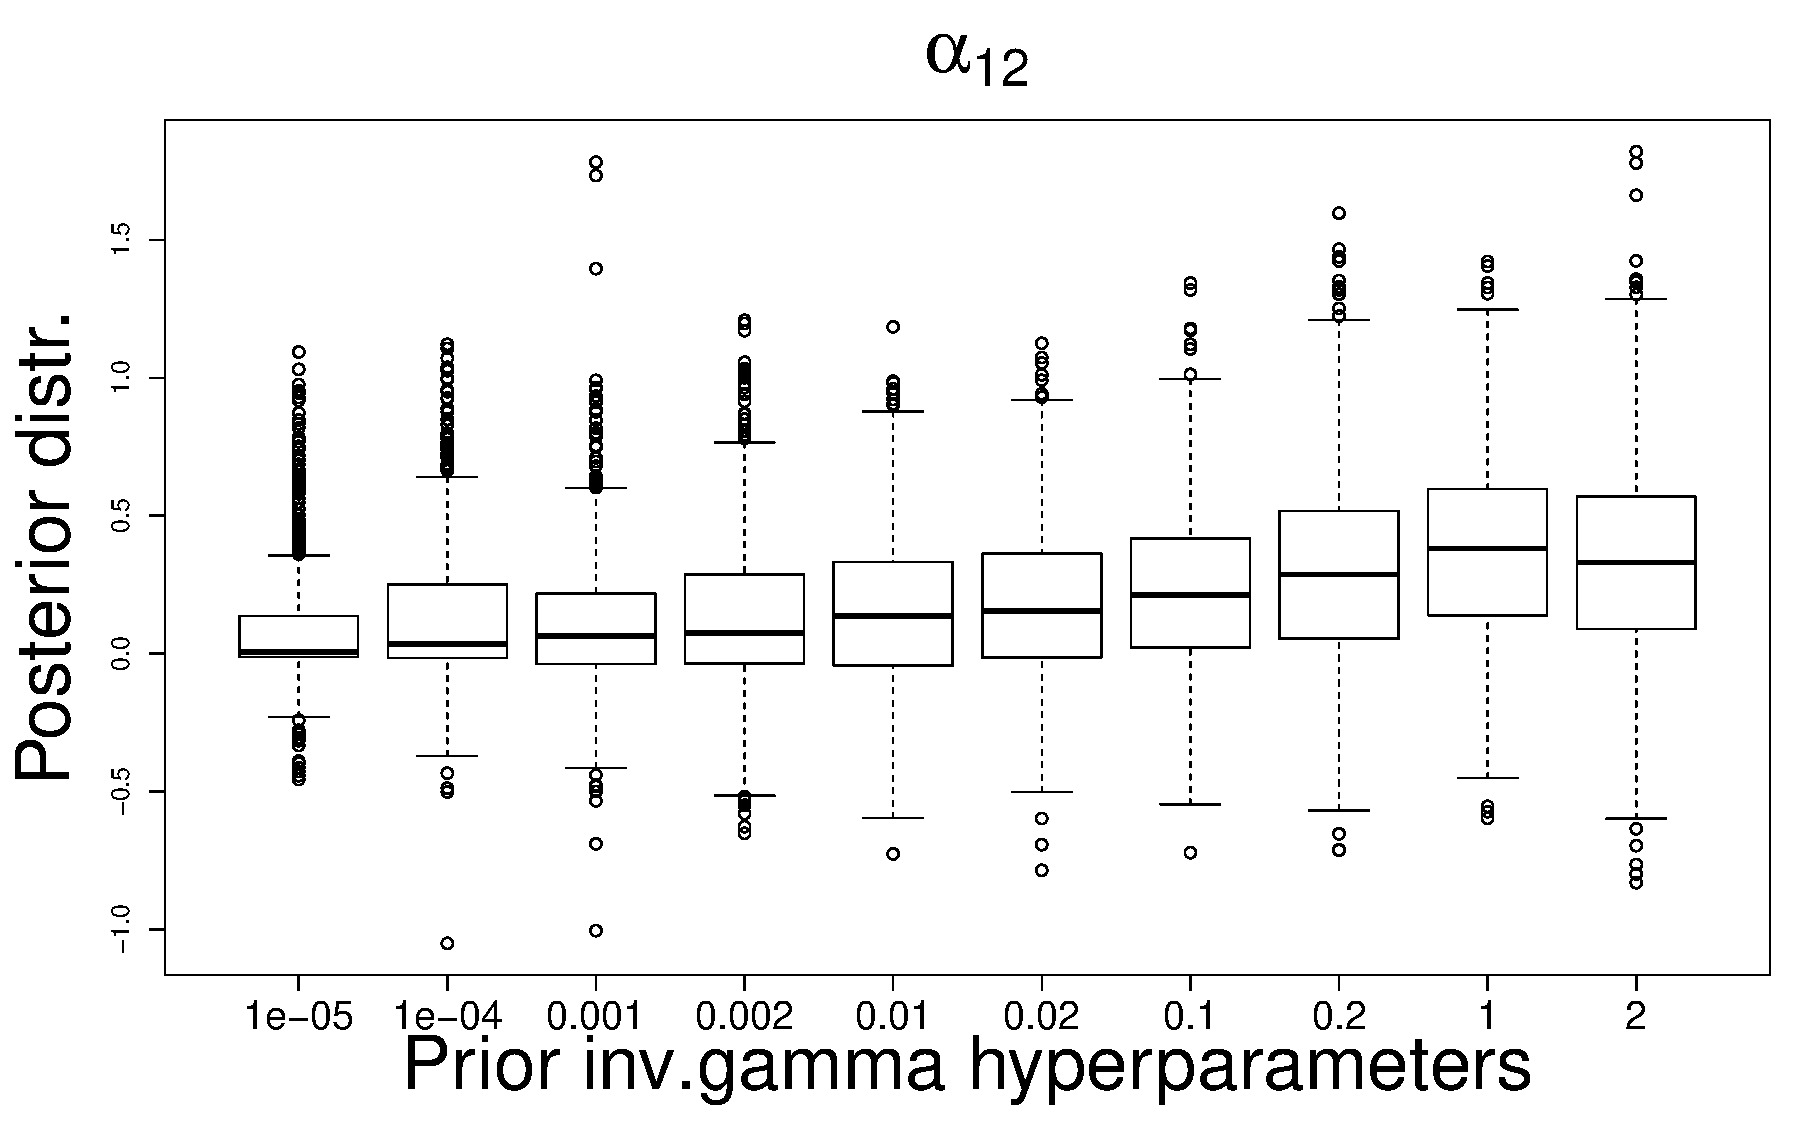
\includegraphics[scale=0.25]{Sensitivity/alpha_12_sensitivity.pdf}\\
\caption{Sensitivity tests for the marginal posterior distributions of of the point abilities parameters $\beta_9, \ldots,\beta_{14}$ and the extra set abilities $\alpha_{10}, \alpha_{12}$ by varying the hyperparameters of the inverse-gamma priors assigned to the parameters: $\tau^2_{\alpha}, \tau^2_{\beta}$. {\tt rjags}, 1000 MCMC iterations, burn-in period of 100 iterations.}
\label{figS4}
\end{figure}

\section*{Set dynamic abilities}

For completeness, we depict in Figure~\ref{fig16} the predictive intervals for the dynamic set abilities (model 11 of Table 2 in the paper).

\begin{figure}
\centering
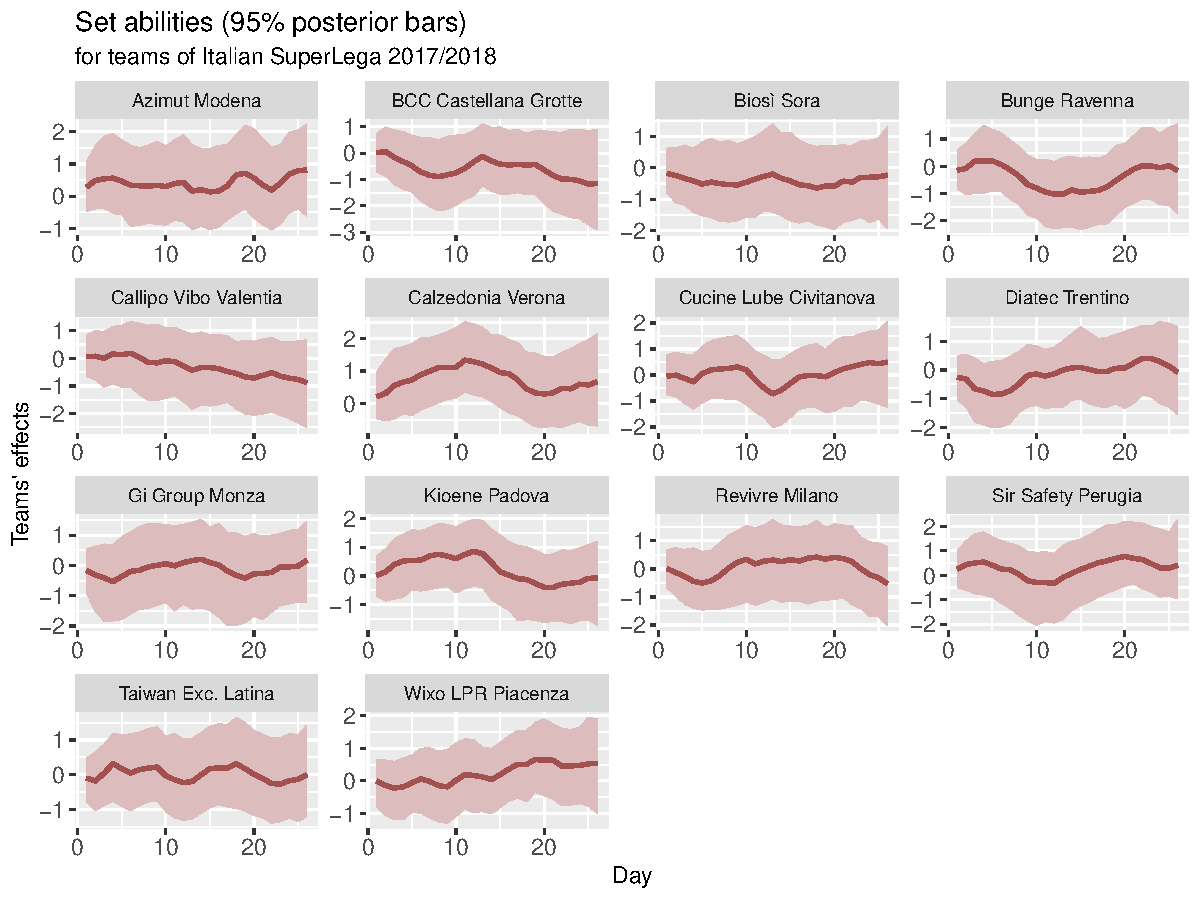
\includegraphics[scale=0.75]{Dynamics/NegBin_ZIP_dynamicset_abilities.pdf}
\caption{Posterior mean and 95\% density interval for the dynamic set abilities parameters $\bm{\alpha}$, Italian SuperLega 2017/2018 (model 11 in Table 2 of the paper).}
\label{fig16}
\end{figure}

\section*{Trace and density plots}

We depict in Figure~\ref{figS6}--\ref{figS7} the trace and the density plots from the MCMC sampling for the parameters: $\mu, \theta, H^{point}, H^{set},\lambda, m$ (\texttt{rjags}, 1000 iterations, burn-in of 100, 3 chains).

\begin{figure}
\centering
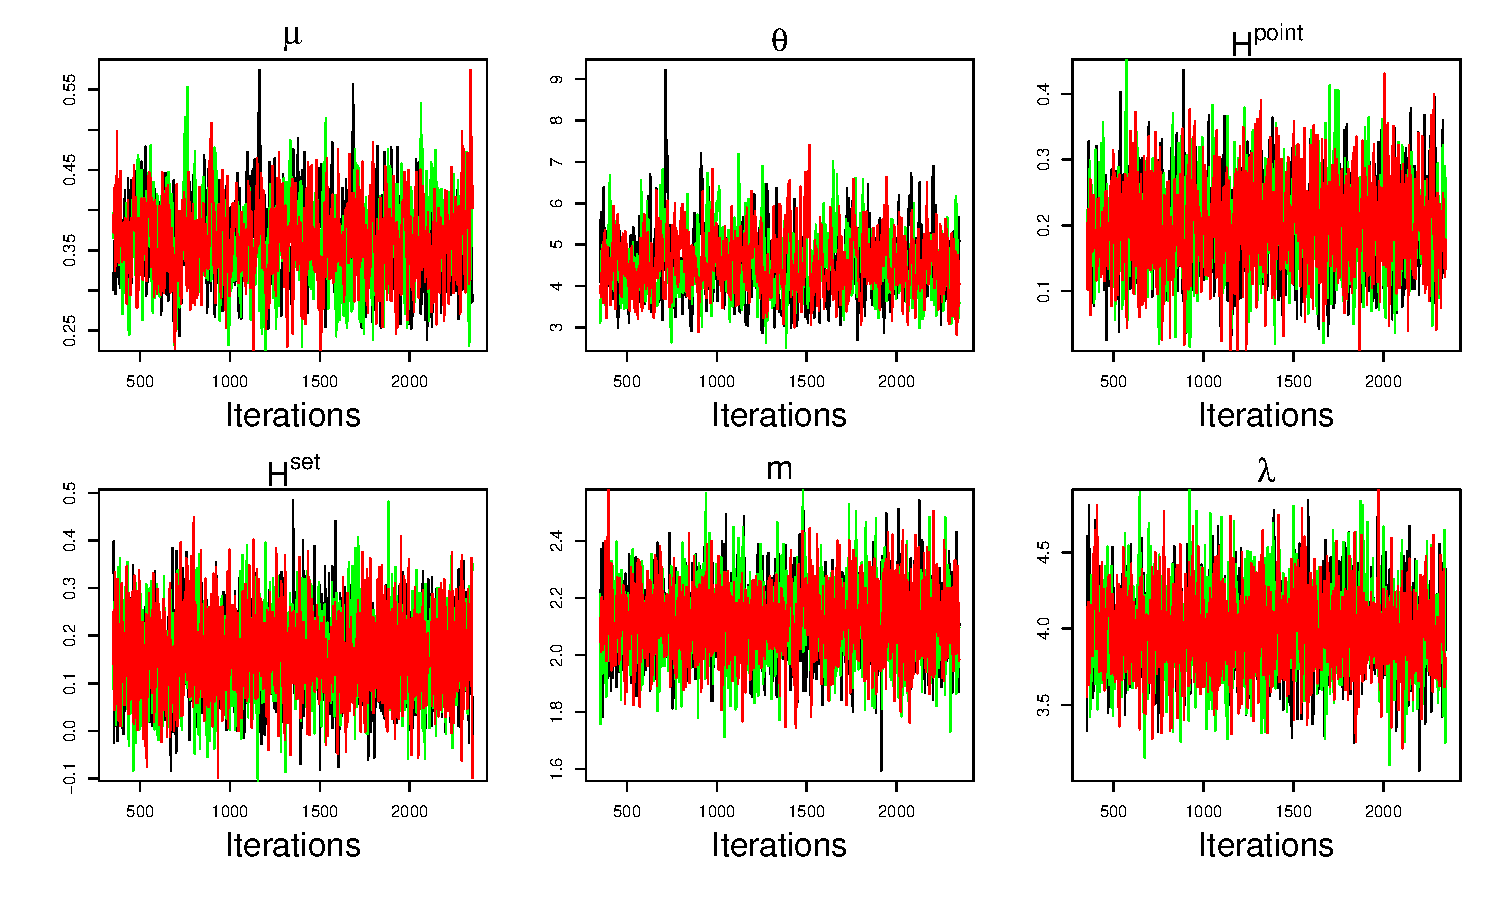
\includegraphics[scale=0.6]{Traceplots/Traceplots.pdf}\\
\caption{Trace plots for the parameters: $\mu, \theta, H^{point}, H^{set},\lambda, m$ (model 9 in the paper).}
\label{figS6}
\end{figure}



\begin{figure}
\centering
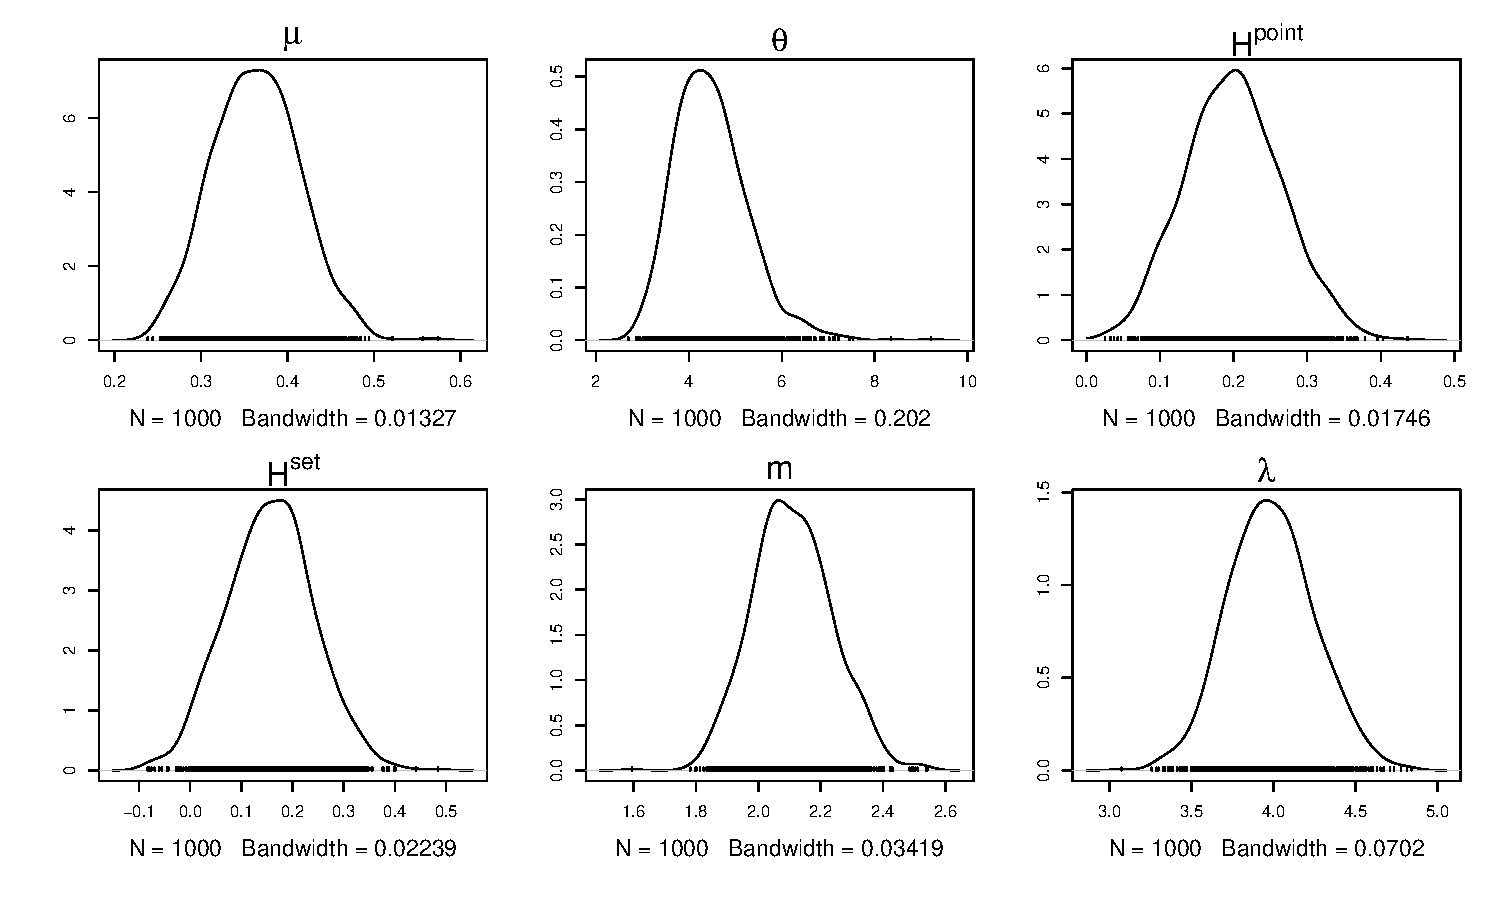
\includegraphics[scale=0.6]{Traceplots/Densplots.pdf}\\
\caption{Density plots for the parameters: $\mu, \theta, H^{point}, H^{set}, m, \lambda$  (model 9 in the paper).}
\label{figS7}
\end{figure}




\end{document}